% updated April 2002 by Antje Endemann
% Based on CVPR 07 and LNCS, with modifications by DAF, AZ and elle, 2008 and AA, 2010, and CC, 2011; TT, 2014; AAS, 2016; AAS, 2020

\documentclass[runningheads]{llncs}
\usepackage{graphicx}
\usepackage{comment}
\usepackage{amsmath,amssymb} % define this before the line numbering.
\usepackage{color}



%%%%%%%%%Add by Lele Chen%%%%%%%%%%%%%%%%%%%%%%

%%%%%%%%%Add by Lele Chen%%%%%%%%%%%%%%%%%%%%%%
\graphicspath{{images/}}
\usepackage{breqn}
\usepackage{multirow}
\usepackage{hhline}
\usepackage{ltablex}
\usepackage{siunitx}
\usepackage{caption}
\usepackage{booktabs}
%\captionsetup[table]{skip = 3pt}
\usepackage{algorithm}
\usepackage{algcompatible}
\usepackage[noend]{algpseudocode}
%%%%%%%%%%%%%%%

%%%%%%%%%Add by Celong Liu%%%%%%%%%%%%%%%%%%%%%%
\usepackage{mathtools}
\usepackage{arydshln}
\DeclarePairedDelimiter{\norm}{\lVert}{\rVert}
\usepackage{capt-of}
\usepackage{float}
\usepackage{wrapfig}
\usepackage{bm}
\usepackage{afterpage}
\usepackage[export]{adjustbox}
\usepackage{amsthm,enumitem}
\def\mathbi#1{\textbf{\em #1}}

\providecommand{\lchen}[1]{\textcolor{blue}{[{\bf #1}]}}
\providecommand{\celong}[1]{\textcolor{cyan}{[{\bf #1}]}}
\providecommand{\zhong}[1]{\textcolor{green}{[{ #1}]}}
\providecommand{\CXu}[1]{\textcolor{red}{[{\bf #1}]}}
\providecommand{\ytian}[1]{\textcolor{green}{[{\bf #1}]}}
%%%%%%%%%Add by Lele Chen%%%%%%%%%%%%%%%%%%%%%%


% INITIAL SUBMISSION - The following two lines are NOT commented
% CAMERA READY - Comment OUT the following two lines
\usepackage{ruler}
\usepackage[width=122mm,left=12mm,paperwidth=146mm,height=193mm,top=12mm,paperheight=217mm]{geometry}



\begin{document}
% \renewcommand\thelinenumber{\color[rgb]{0.2,0.5,0.8}\normalfont\sffamily\scriptsize\arabic{linenumber}\color[rgb]{0,0,0}}
% \renewcommand\makeLineNumber {\hss\thelinenumber\ \hspace{6mm} \rlap{\hskip\textwidth\ \hspace{6.5mm}\thelinenumber}}
% \linenumbers
\pagestyle{headings}
\mainmatter
\def\ECCVSubNumber{100}  % Insert your submission number here


%%%%%%%%% TITLE
\title{Talking-head Generation with Individual and Rhythmic Head Motion}

% INITIAL SUBMISSION 
%\begin{comment}
\titlerunning{ECCV-20 submission ID \ECCVSubNumber} 
\authorrunning{ECCV-20 submission ID \ECCVSubNumber} 
\author{Anonymous ECCV submission}
\institute{Paper ID \ECCVSubNumber}
%\end{comment}
%******************

% CAMERA READY SUBMISSION
\begin{comment}
\titlerunning{Abbreviated paper title}
% If the paper title is too long for the running head, you can set
% an abbreviated paper title here
%
\author{First Author\inst{1}\orcidID{0000-1111-2222-3333} \and
Second Author\inst{2,3}\orcidID{1111-2222-3333-4444} \and
Third Author\inst{3}\orcidID{2222--3333-4444-5555}}
%
\authorrunning{F. Author et al.}
% First names are abbreviated in the running head.
% If there are more than two authors, 'et al.' is used.
%
\institute{Princeton University, Princeton NJ 08544, USA \and
Springer Heidelberg, Tiergartenstr. 17, 69121 Heidelberg, Germany
\email{lncs@springer.com}\\
\url{http://www.springer.com/gp/computer-science/lncs} \and
ABC Institute, Rupert-Karls-University Heidelberg, Heidelberg, Germany\\
\email{\{abc,lncs\}@uni-heidelberg.de}}
\end{comment}
%******************
\maketitle

%%%%%%%%% ABSTRACT
\begin{abstract}
Given a conditioned modality (e.g., speech audio signal, video frames), generating a talking-head video synchronized with the given condition while moving the head naturally is challenging. When people delivery a speech, we naturally move heads, and this rhythmic head motion conveys linguistic information. 
While remarkably successful, existing works either generate still talking-face videos or rely on landmark/video frames as sparse/dense mapping guidance to generate head movements, which leads to unrealistic and uncontrollable video synthesizing. 
To overcome the limitation, we propose a 3D aware module to model the head motion and facial expression explicitly and a matching scheme along with a texture preserving GRU module to model the temporal dependencies. Compared to a direct condition-to-image approach, our approach avoids overfitting to the subjects in the training data, which leads to a much better generalization capability. Meanwhile, our system is compatible with the adversarial fine-tuning to further improve the video quality. Thoughtful experiments on two standard benchmarks demonstrate that our method achieves significantly better results than the state-of-the-art methods in both quantitative and qualitative comparisons.  

%we propose a novel talking-head generation task with natural head movements. Instead of learning a direct mapping from given driving modality (e.g. an arbitrary speech signal or a reference video, etc.) to video frames, we propose a novel method to generate talking-head video by leveraging the 3D modeling with generative model to produce a realistic output video in which the facial expressions of the speaker is synchronized with the given conditioned modality, while moving their head naturally. Compared to a direct condition-to-image approach, our approach avoids overfitting to the identities in the training dataset, which leads to a much better generalization capability. Meanwhile, our system is compatible with the adversarial fine-tuning to further improve the video quality. Thoughtful experiments on two standard benchmark datasets demonstrate significantly better results obtained by our method than the state-of-the-art methods in both quantitative and qualitative comparisons. As an attempt to bridge the gap between still taking-face generation and talking-head generation, we propose a novel video generation framework aiming at disentangling individual head motion and generating talking-head with controllable head motion. 
  
\end{abstract}


%%%%%%%%% BODY TEXT
\section{Introduction}
\label{sec:intro}

%\CXu{
%A general formula to write the Introduction section of your paper.
%1. BACKGROUND: Briefly describe the background. Motivate this work.
%2. PROBLEMS: State the (new) problem you are addressing in this paper and why this is important.
%3. CHALLENGES: Describe the challenges. Briefly mention existing works, how they address the challenges, and what they fail to address.
%4. SOLUTION: Introduce our approach
%5. NOVELTY: Contrast ours to existing works to highlight our contribution
%6. ORGANIZATION (optional): The rest of the paper is organized as the following.
%}

%\CXu{Introduction is not good. There lacks a clear flow/story. Shall we separate the concepts of ``talking-face'' and ``talking-head''? Talking-face: head is still, or not considered explicitly. Talking-head: aim to manipulate head movement; it can come from a driving modality, e.g., another talking head, 3D pose, or be generated based on short-term talking characteristics. Therefore, you can group literature into one of the two sets and make the comparison. Of course, you will need to say why we need to generate head motion: 1) it helps to comprehend speech; 2) the value in terms of computer vision, e.g., the model needs to have a 3D-aware capability?}
%BACKGROUND and Motivation
People spontaneously emit head movements when we speak, which complement speech and add non-verbal information that helps the audience comprehend what we say~\cite{cassell1999speech,ginosar2019gestures}. Modeling the dynamics of a talking-head video and then generating controllable talking-head video conditioned on a driven modality (e.g., audio speech, landmarks, RGB images) is a valuable problem in computer vision. For example, by modeling the head motion and facial expressions, we can generate controllable talking-head videos, which can benefit the research of adversarial attacks in security or provide more training samples for supervised learning approaches. Solving this problem is also crucial to real-world applications, e.g., generating vivid talking-head videos that convey the conditioned speech can enhance speech comprehension while preserving privacy, or build assistive devices for hearing impaired people. 

\begin{figure}[t]
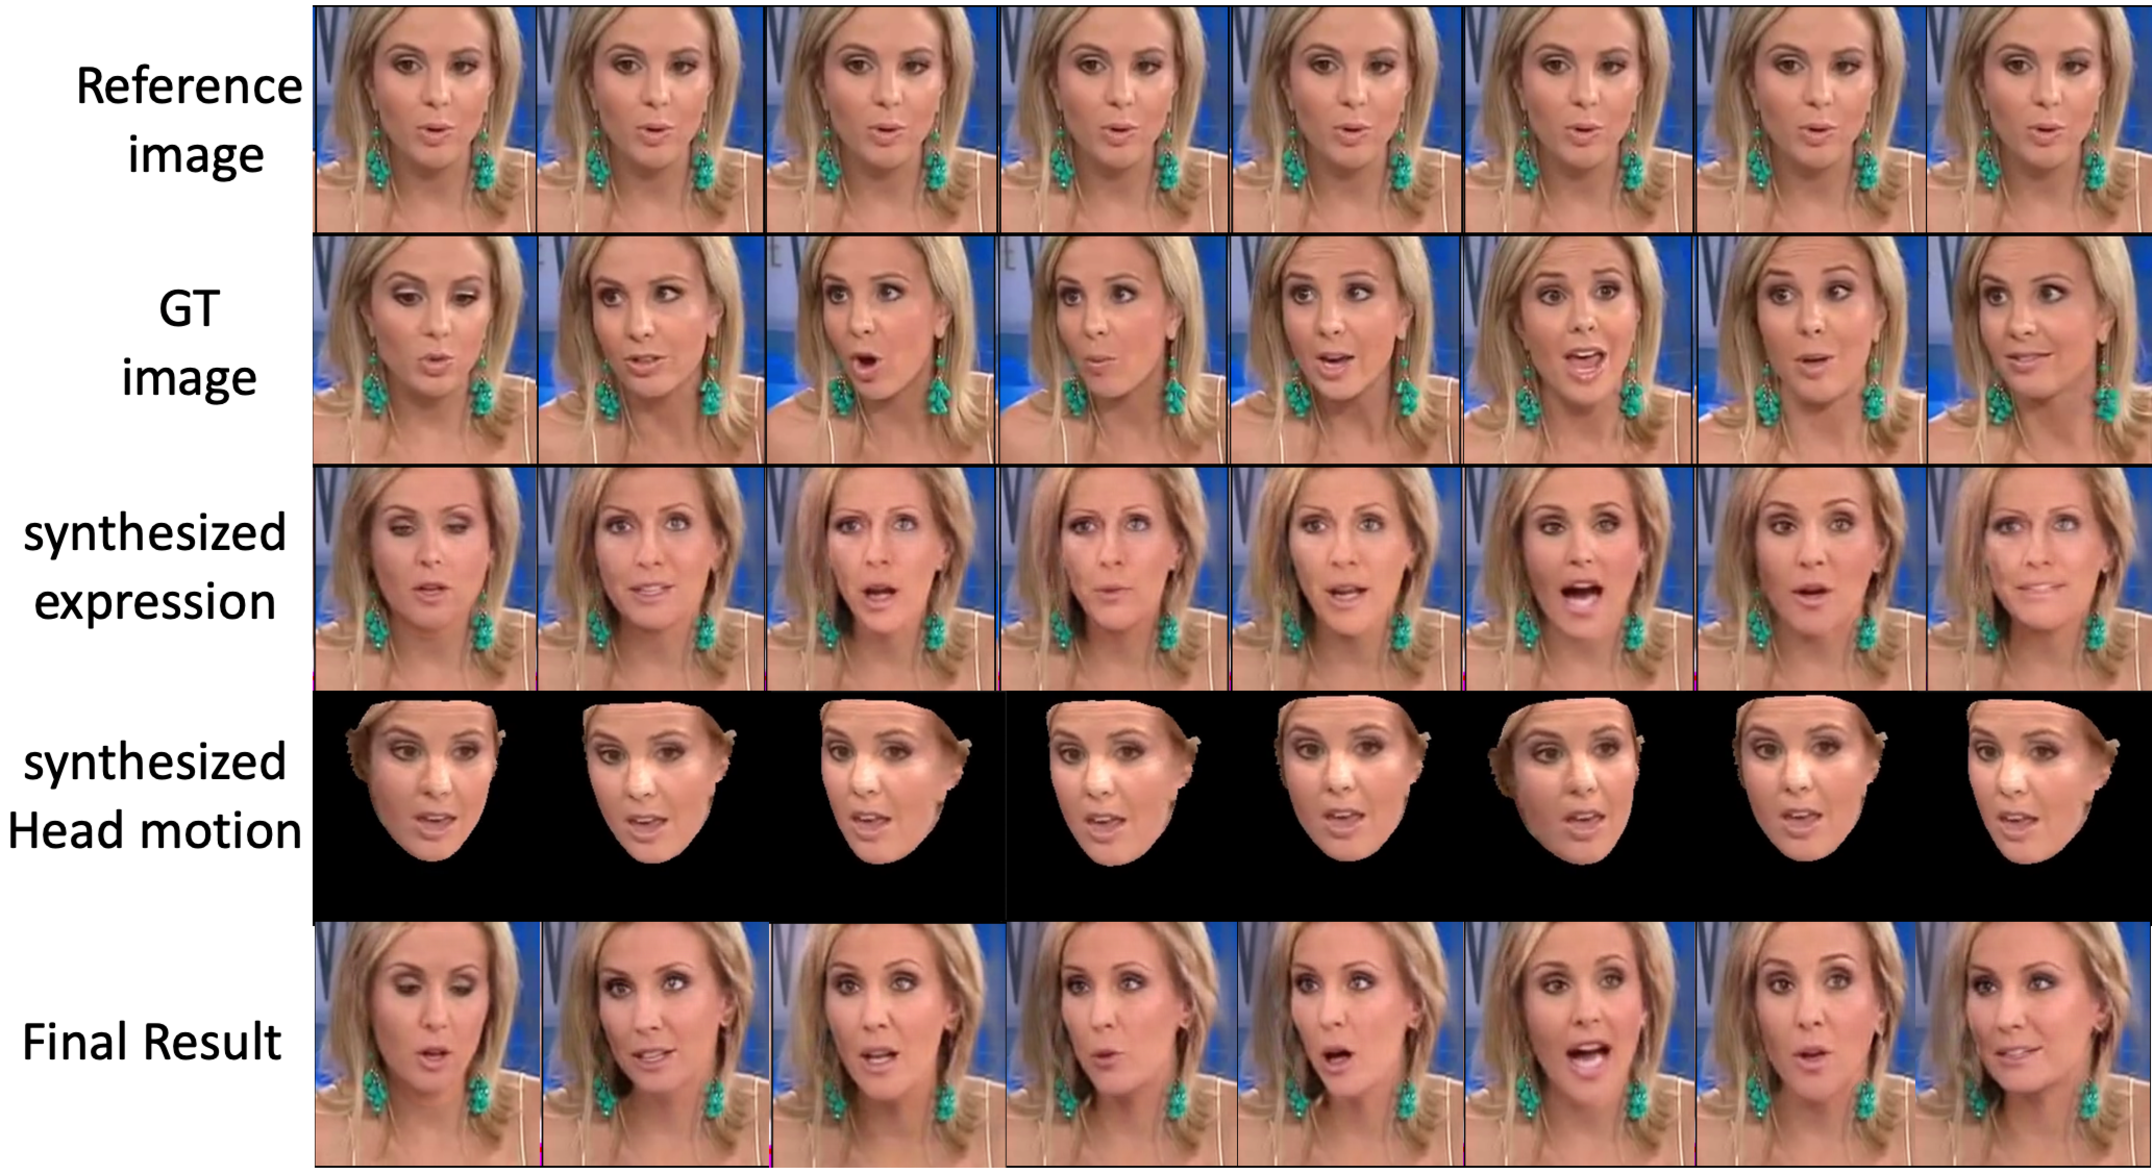
\includegraphics[width= \linewidth]{latex/images/teaser.pdf}
\caption{The illustration of our approach. Given a short video, we can explicitly model the head motion and facial expression in a disentangled manner.}
% \vspace{-6.5mm}
\label{fig:teaser}
\end{figure}


%PROBLEMS and some related works
We humans can infer the visual prosody from a short conversation with the speaker~\cite{munhall2004visual}. Drawing inspiration from the human perception, in this paper, we consider such a task: given a short video (e.g., 3 seconds) of the target subject and an arbitrary reference speech audio recording or reference video from a different subject, learning the individual head motion from the 3-second video and generating a photo-realistic talking-head video of the target subject that conveys the conditioned audio or video. The synthesized subject should have natural lip synchronization and smooth transition while moving the head with natural and rhythmic head motion. Similar problems (e.g., talking-face generation~\cite{chung2017you,zhou2019talking,ijcai2019-129,vougioukas2019realistic,chen2019hierarchical} and~\cite{wiles2018x2face,zakharov2019few,wang2018fewshotvid2vid}) have been explored recently. However, several challenges on how to explicitly use the given video and model the head motion remain unsolved. And we discuss our technical contributions concerning each challenge. 

%CHALLENGES

%challenge 1: convoluted features.
The deformation of talking-head consists of his/her intrinsic subject traits, head movements and facial expressions, which are highly convoluted. This complexity stems not only from modeling face regions, but also from modeling head motion and background. while the synthesized talking-face conveys the input audio signal, previous talking-face methods~\cite{Chung18b,wiles2018x2face,zhou2019talking,chen2018lip,ijcai2019-129,chen2019hierarchical} omit the head motion modeling thus can only generate still talking-face with expressions under a fixed facial alignment. Other talking-head generation methods~\cite{zakharov2019few,wang2018fewshotvid2vid,wang2018vid2vid,wang2018high,wiles2018x2face} are able to synthesize moving-head videos by replying on input facial landmarks or RGB video frames as the guidance to infer the convoluted head motion and facial expressions. However, they do not model head motion and facial expression (see Fig.~\ref{fig:teaser}) explicitly (e.g., control facial expression with speech audio signal), thus fail to output a controllable talking-head video, which we argue greatly limits their use. For example, we can not use audio speech to drive those talking-head generation methods since the head motion is missing. To address the convoluted deformation problem, we propose a simple but effective method to decompose the identity appearance, head motion, and facial expression and generate controllable talking-head videos either conditioned upon audio signal or RGB images.     

%challenge 2: 3 seconds video.
Another challenge is exploiting the information contained in reference images/video. While the few-shot generation methods~\cite{zakharov2019few,wang2018fewshotvid2vid,liu2019few} learn to synthesize high-quality videos of unseen subjects by leveraging $K$ reference images, they only utilize the global appearance information. There is much valuable information other than appearance. For example, we can infer the individual characteristics in head movement by leveraging the given short video. Thus, we propose a novel method to extrapolate rhythmic head motion based on the input short video while preserving a few characteristics of the individual head motion. This extrapolated head motion can be used in speech-driven talking head generation task as the head motion guidance. Furthermore, we propose a matching scheme to utilize the given video to smooth the facial movement transition and stabilize the backgrounds.

%challenge 3: 3D 
People are sensitive to any temporal discontinuities (e.g., subtle artifacts and perceptual identity changes) in a synthesized video, which is hard to avoid in GAN-based methods. 3D graphics modeling has been introduced by~\cite{Fried19,kim2018deep} in GAN-based methods due to its stability. In this paper, we employ the 3D modeling along with a novel temporal Texture Aware Gated Recurrent Unit (\textit{TP-GRU}) to model the temporal dependencies at the generation stage to alleviate the temporal discontinuities caused by head motion, facial expressions or the overfitting problem.

%summary
Combining above features, which are designed to overcome limitations of existing methods, our framework can generate talking-head video with natural head motion that conveys the given input condition. We conduct extensive experimental validation with comparisons to various state-of-the-art methods on several benchmark datasets (e.g., VoxCeleb2~\cite{Chung18b}, LRW~\cite{Chung16}, and VoxCeleb1~\cite{Nagrani17} datasets ) under several different settings (e.g., audio to video, landmark to video, and few-shot learning). Experimental results show that the proposed framework effectively addresses the limitations of existing talking-head generation methods.

\section{Related Work}
\label{sec:related}
In this section, we first briefly survey related work on the talking-face/head generation task. Then we discuss the related work of each technique used in our model. %\CXu{I don't like the way you organize the related work. I think a better way and a logic way is to focus on the related work on talking face/head generation. You should organize the related literature into categories, e.g., graphics-based or data driven based etc. Mention each important related paper, and their limitations.}

%\CXu{I don't know the purpose of this paragraph.} \noindent \textbf{Generative models} \quad Our proposed approach is based on conditional Generative adversarial network~\cite{mirza2014conditional, goodfellow2014generative,mao2017least}. The talking-head video synthesis requires human interpretable controls (e.g. sketches~\cite{chen2019hierarchical,zakharov2019few}, audio~\cite{zhou2019talking, ijcai2019-129} and RGB image~\cite{wiles2018x2face}), thus, rather than from noise distribution~\cite{goodfellow2014generative,walker2016uncertain,karras2019style, sangkloy2017scribbler,zhu2019dm,huang2019generative}, we synthesize the target videos directly based on user input data, which offers more control over the generated results. \noindent \textbf{Talking-face/head Synthesizing} \quad
\subsection{Talking-face/head Image Generation}
\label{subsec:talking-syn}
The success of graphics-based approaches has been mainly limited to synthesizing talking-head videos for a specific person~\cite{garrido2015vdub,bregler1997video,chang2005transferable,liu2011realistic,suwajanakorn2017synthesizing}. For instance, Suwajanakorn et al.~\cite{suwajanakorn2017synthesizing} produce photo-realistic videos by a speech-driven approach. While it can synthesize fairly accurate lip-synced videos, it requires the target audio speech similar to the original speaker and a large amount of video footage of the target person. Moreover, this method can not be generalized to an unseen person due to the rigid matching scheme. More recently, video-to-video translation has been shown to be able to generate arbitrary faces from arbitrary input data. While the synthesized video conveys the input speech signal, the talking-face generation methods~\cite{chung2017you,zhou2019talking,ijcai2019-129,Vougioukas2019,chen2019hierarchical} can only generate facial expressions without any head movements under a fixed alignment since the head motion modeling has been omitted. Talking-head methods~\cite{zakharov2019few,chen2019hierarchical,wiles2018x2face} are able to generate high-quality videos with convoluted facial expression and head motion. However, due to the lack of explicit head motion modeling, these methods can not generate controllable video, e.g., using audio to drive the generation. 

\subsection{Related Techniques }
\label{subsec:related_tec}
\noindent \textbf{Head Motion Modeling} \quad
One challenging problem of talking-head video generation is head motion modeling, which has been ignored by previous works~\cite{pumarola2019ganimation,vougioukas2019realistic,chung2017you,ijcai2019-129,zhou2019talking}. However, people are sensitive to unnatural head motion and can easily tell the fake video if it is a still head with facial expressions. Some works~\cite{zakharov2019few,wang2018fewshotvid2vid,wiles2018x2face} employ facial landmarks or face images to establish a sparse or dense mapping to generate images with desired head motion. For example, Wiles et al.  create a dense mapping between the image paired with target pose and a embedded face of reference subject and sample the pixels from the embedded face using the estimated mapping. However, the facial expressions and head movements are convoluted in the image and this method can not generate facial expressions or head movements separately. Fried et al.~\cite{Fried19} explore generating images with different head poses, but their method can only retrieve poses that exist in their footage database, which limits their method as a video editing method instead of a video generating method since they can not generate new head motion for feature frames. We explicitly model the head motion and facial expression in a disentangle manner and propose a method to extrapolate rhythmic head motion for future frames to enable audio-driven talking-head generation.  % In this work, we propose a new fundamental problem in taking-head generation tasks: modeling the head motion while synthesis videos from other conditioned user input data. And we discussed our head motion extrapolation in the method section, which, to the best of our knowledge, is the first paper consider head motion modeling in talking-head video generation task. 
%controlling the facial expression and head model separately, 

\noindent \textbf{Attention Mechanism} \quad Attention mechanism, proposed by Vondrick et al.~\cite{vondrick2016generating}, has been well explored in image/video generation task~\cite{vondrick2016generating,wang2018vid2vid,pumarola2019ganimation,chen2019hierarchical}. For instance, Pumarola et al.~\cite{pumarola2019ganimation} compute the final output image by $\hat{\mathbf{I}} = (1 - \mathbf{A}) * \mathbf{C} + \mathbf{A} * \mathbf{I}_r $, where $\mathbf{I}_r$, $\mathbf{A}$ and $\mathbf{C}$ are input reference image, attention map and color mask, respectively. The attention map $\mathbf{A}$ indicates to what extend each pixel of $\mathbf{C}$ contributes to the output image $\hat{\mathbf{I}}$. However, this attention mechanism is not working if there exits large deformation between reference frame $\mathbf{I}_r$ and target frame $\hat{\mathbf{I}}$. Wang et al.~\cite{wang2018high} use estimated optic flow to warp the $\mathbf{I}_r$ to align with $\hat{\mathbf{I}}$, which is computationally expensive and can not estimate the rotations in talking-head videos. In this paper, we propose a 3D manipulation solution to better tackle the misalignment problem caused by head motion. 

\noindent \textbf{Temporal Dependency Modeling} \quad 
One of the main differences between the image-to-image generation and video generation is the temporal-dependency modeling, which is overlooked by previous talking-head generation works~\cite{chung2017you,wiles2018x2face,zakharov2019few,chen2018lip}. It is worth to mention that Song et al.~\cite{ijcai2019-129} compare different conditional video generation schemes and propose a recurrent frame generation scheme. However, their recurrent unit is limited to refine the feature vector (lack of spatial information), which failed to consider the temporal smoothness in the generation stage. In this paper, we propose a novel \textit{TP-GRU} unit to model the temporal dependencies at the generation stage. Furthermore, we propose a novel matching scheme to leverage the given video frames to contribute to the synthesized video frames in the generation stage to better model the temporal consistency.
\begin{figure*}[ht]
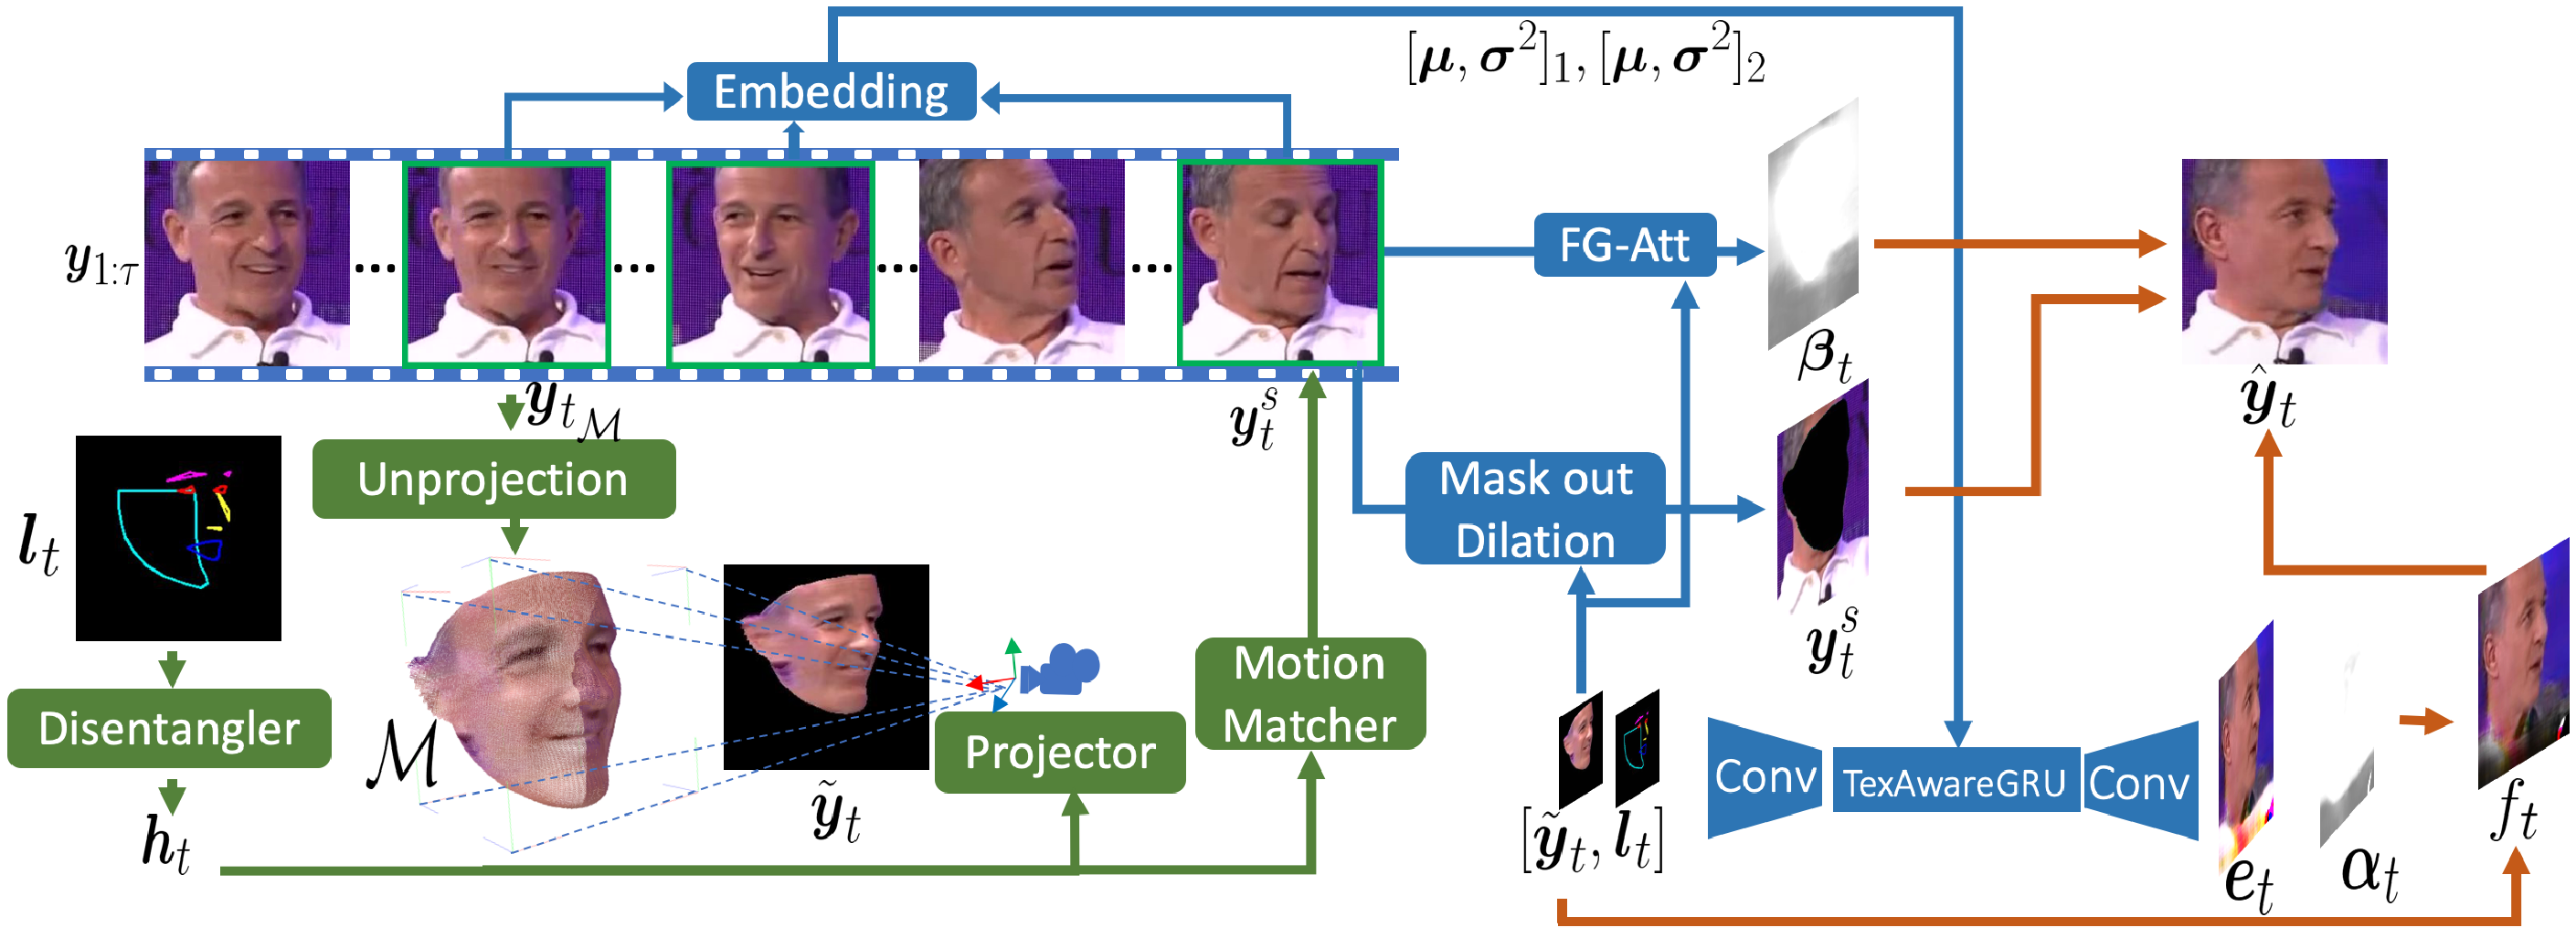
\includegraphics[width=1.0 \linewidth]{latex/images/main.pdf}
\caption{The overview of the generator framework in the training stage, which consists of three modules: green, blue and orange part are the \textit{3D Aware} Module, the \textit{TP-GRU} module and the \textit{AttBuilder} module, respectively.}
% \vspace{-6.5mm}
\label{fig:main}
\end{figure*}

\section{Method}
\label{sec:method}

%\CXu{I made a quick pass of the next two sections and fixed some obvious errors in notation. Someone should check the notations carefully.}


\subsection{Problem Formulation}
\label{subsec:problem_formulation}

%\CXu{Combine the next two paragraphs into one *short* paragraph. Simply tell the problem settings in *training* only. Point the readers to read the next section (Sec. 4) for different driven modalities in inference.}
%\CXu{$--->$ Start from here:}
We introduce a neural approach for talking-head video generation leveraging temporal modeling and 3D manipulation. Our approach takes as input sampled video frames, $\mathbi{\mathbi{y}}_{1:\tau} \equiv \mathbi{\mathbi{y}}_1,...,\mathbi{\mathbi{y}}_{\tau}$, of the target subject and a driving condition, $\mathbi{\mathbi{x}}_{\tau+ 1:T}  \equiv \mathbi{\mathbi{x}}_{\tau + 1},...,\mathbi{\mathbi{x}}_T$ (e.g., a speech signal or a sequence of facial landmarks, etc.), and synthesizes target video frames, $\hat{\mathbi{y}}_{\tau + 1:T}  \equiv \hat{\mathbi{y}}_{\tau + 1}, ...,\hat{\mathbi{y}}_T$, that convey the given condition with realistic head movements. During training, we transfer the input condition, $\mathbi{\mathbi{x}}_{\tau+ 1:T}$, to the 3D facial landmark representation, $\mathbi{l}_{\tau+1: T}$~\cite{feng2018joint}, leading the sequential generative model $F$ given by:
\begin{equation}
\begin{aligned}
\hat{\mathbi{y}}_{ \tau+1:T} =  F( \mathbi{y}_{1:\tau},\mathbi{l}_{\tau+1:T}  )  \enspace.
\end{aligned}
\label{eq:training}    
\end{equation}
% \CXu{What is $F$?}
We discuss the network architecture and training details in this section, and the inference process with driven conditions is in Sec.~\ref{sec:infer}.

\subsection{Method Overview}
\label{subsec:overview}

The proposed framework (see Fig.~\ref{fig:main}) aims to exploit the information in $\mathbi{y}_{1:\tau}$ and maps the transferred 3D landmarks, $\mathbi{l}_{\tau+1:T}$, to a sequence of generated video frames, $\hat{\mathbi{y}}_{ \tau+1:T}$. The framework consists of three modules. The \textit{3D Aware} module (Fig.~\ref{fig:main} green part) decomposes the head motion and facial expressions from $\mathbi{l}_{\tau+1:T}$ and generates different 3D projections as the network input. The network learns a dense mapping from the projection input. Comparing to landmark-only input~\cite{zakharov2019few,wang2018fewshotvid2vid,wang2018high}, it can alleviate the overfitting problem and make training converge faster. The \textit{TP-GRU} module (Fig.~\ref{fig:main} blue part) is proposed to explicitly fuse the global texture feature with facial expression and head pose feature while considering the temporal-dependency modeling. Comparing to image-level generation methods~\cite{chung2017you,pumarola2019ganimation,zhou2019talking,zakharov2019few,wang2018high}, our \textit{TP-GRU} module can synthesize videos with natural lip synchronization and smoother transition. The \textit{AttBuilder} module (Fig.~\ref{fig:main} orange part) is proposed to stabilize the background and better preserve the individual appearance at the end of the generation. 


% \CXu{$<--$ Goes to the next three sections, only if needed. Otherwise, delete.}

\begin{figure}
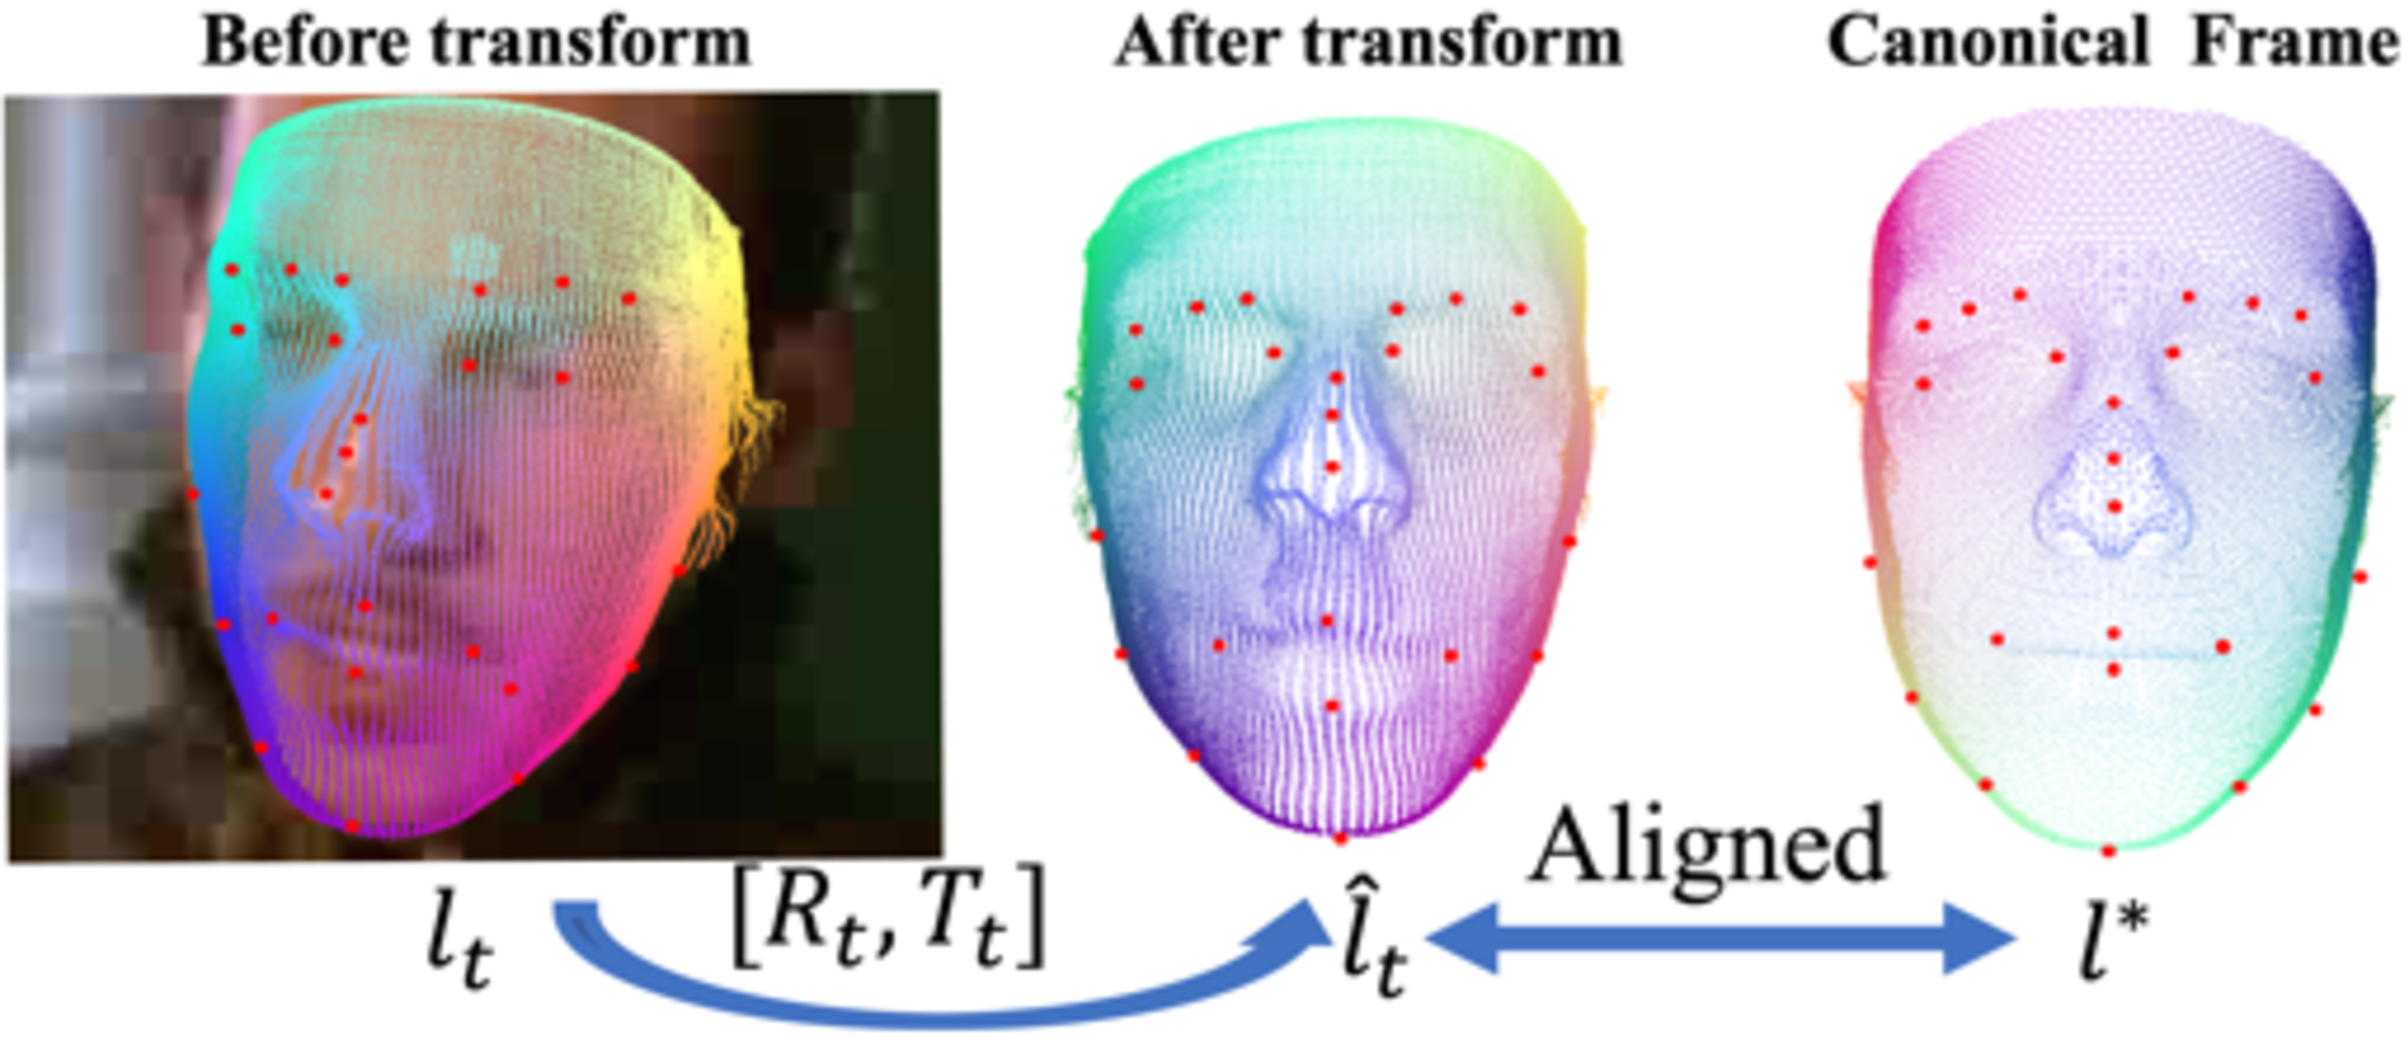
\includegraphics[width=0.8 \linewidth]{latex/images/RT_reduce.pdf}
\caption{The movement vector extraction. The top left is image frame at time step t, the bottom left figure shows the transformation matrix calculation from $\mathbi{l}_t$ to $\mathbi{l}^*$. The right side figure shows how to apply the computed $[\mathbf{R},\mathbf{T}]_t$ to $\mathbi{l}_t$ to get frontalized landmark $\hat{\mathbi{l}}_t$.}
% \vspace{-6.5mm}
\label{fig:rt_compute}
\end{figure}


% For each video sequence, we choose the most visible frame from $y_{1:\tau}$ and feed it to a pretrained U-net structure network~\cite{feng2018joint} to unproject it to 3D mesh $\mathcal{M}$. Then we randomly select $K$ images from the input $\tau$ continuous frames as references and use an \textit{embedding network} to embed the references into an appearance vector $\mathbi{z}_{y} \in \mathbb{R}^{512}$. Then, at each time step $t$, we disentangle the head motion, $\mathbi{h}_t \in \mathbb{R}^{6}$ from the given 3D facial landmark $\mathbi{l}_t \in \mathbb{R}^{68 \times 3}$ using \textit{motion disentangle} module and manipulate the 3D mesh $\mathcal{M}$ using the computed head motion $\mathbi{h}_{t}$ to get a new projection $\tilde{\mathbi{y}}_t$. The projected image $\tilde{\mathbi{y}}_t$ is featured by the perfectly aligned texture information despite the facial expressions since it is computed by target $\mathbi{h}_t$. 

% We feed the projected image and converted facial landmark image pair $[\tilde{\mathbi{y}}_t \in \mathbb{R}^{H\times W \times C}, \mathbi{l}_t \in \mathbb{R}^{H\times W \times C}] $ into convolutional layers to get the encoded expression feature $\mathbi{e}_t \in \mathbb{R}^{\frac{H}{64} \times \frac{w}{64} \times 512} $ and then fuse it with the embedded appearance vector $\mathbi{z}_y$ in \textit{TexAwaredGRU} module. Comparing to~\cite{zakharov2019few}, which only encodes landmark, our $\tilde{\mathbi{y}}_{t}$ provides a strong prior of the appearance feature at the encoding stage, which speeds up the convergence of the model and alleviates the overfitting problem caused by AdaIN normalization. 

% Then after several convolutional layers with upsampling, we obtain foreground image $\mathbi{f}_t \in \mathbb{R}^{H\times W \times C}$. The disentangled head motion $\mathbi{h}_t$ can also be used to match a similar frame $\mathbi{sy}_{t} \in \mathbb{R}^{H\times W \times C}$ from the sampled images $\mathbi{y}_{1:K}$ by \textit{motion matcher}. The matched frame $\mathbi{sy}_{t}$ is featured in two perspective: the background region is almost aligned with target image $\mathbi{y}_{t}$ and the deformed region compared with foreground $\mathbi{f}_t$ is the place that need to be generated. We use a FG-Att block to generate a learnable foreground-background attention $\boldsymbol{\beta}_t \in \mathbb{R}^{H\times W \times 1}$. With the computed foreground $f_t, \boldsymbol{\beta}_t$ and background $\mathbi{sy}_{t}$, we get the final synthesized image $\hat{\mathbi{y}}_t \in \mathbb{R}^{H\times W \times C}$.

\subsection{\textit{\textbf{3D Aware}} Module}
\label{subsec:3d_man}
%\ytian{whether it is better to add one sentence to describe input/output and the goal of the module?}
% We introduce the \textit{3D Aware} Module in the following three components: 
 \noindent {\bf{Motion Disentangler}}\indent Besides the temporal-dependency modeling and expression synthesizing, a key difference between still image generation and talking-head video generation is natural head movements, which should be consistent with the target subject's individual characteristics. However, we observe that 3D facial landmarks are not only conditioned on head movements but also carry annoying uncontrollable facial expression information. To disentangle head motions from a given 3D landmark $\mathbi{l}_t$, we introduce a motion disentangler, which takes 3D landmark $\mathbi{l}_t$ at each time step $t$ and disentangle it into head motion $\mathbi{h}_{t}$ and facial expression $\hat{\mathbi{l}}_{t}$. That is:
\begin{equation}
\begin{aligned}
{\mathbi{h}}_{t}, \hat{\mathbi{l}}_{t}  = \textit{disentangler} ( \mathbi{l}_{t} )  \enspace.
\end{aligned}
\label{eq:disentangle}    
\end{equation}
%However, the 3D landmark vector $\mathbi{l}_{1:\tau}$ contains many head-movement-non-correlated noise (e.g. facial expressions), and makes  \textit{disentangler} hard to extract head movement representations.
To simplify this problem, rather than modeling the head motion problem in 3D landmark space $\mathbb{R}^{68 \times 3}$, we learn the head movements in linear algebra space. At each time step $t$, we compute the transformation matrix $[\mathbf{R},\mathbf{T}]_t \in \mathbb{R}^{6}$  to represent $\mathbi{h}_{t}$. That is:
\begin{equation}
\begin{aligned}
{\mathbi{h}}_{t} \thickapprox [{\mathbf{R}},{\mathbf{T}]}_{t} \enspace,
\end{aligned}
\label{eq:headmovement2}    
\end{equation}
where we ignore the camera motion and assume the synthesized translation matrix is the head motion vector.
Specifically, we compute the rigid transformation $[\mathbf{R},\mathbf{T}]_t$ from the paired face landmark $\mathbi{l}_t$ to the canonical 3D facial landmark $\mathbi{l}^*$, which is $\hat{\mathbi{l}}_t = \mathbf{R}_t   \mathbi{l}_t + \mathbf{T}_t$. Fig.~\ref{fig:rt_compute} illustrates above procedure. We can find that after transformation, the head movement information is removed, and the resultant $\hat{\mathbi{l}}_t$ only carries the facial expression information, which is correlated with the input condition $\mathbi{x}_t$. To avoid the noise caused by non-rigid deformation, we select 27 points (marked as red points in Fig.~\ref{fig:rt_compute}), which contain less non-rigid deformation.
 
\lchen{ \noindent {\bf{3D Unprojection}}\indent Here, we assume that the image with frontal face contains the most face texture information. Given a short reference video sequence $\mathbi{y}_{1:\tau}$, we compute the head rotation $\mathbf{R}_{1:\tau}$ and choose the most visible frame $\mathbi{y}_{t_{\mathcal{M}}}$ with minimum rotation such that $\mathbf{R}_{t_{\mathcal{M}}} \rightarrow 0$. Then we feed it to an unprojection network to unproject it to 3D mesh $\mathcal{M}$. The Unprojection network is a U-net structure network~\cite{feng2018joint} and we pretrain it on  300W-LP~\cite{zhu2016face} dataset to transfer the input RGB image into position map image. After pretrianing, we fix the weight and use it to transfer the input image $\mathbi{y}_{t_{\mathcal{M}}}$ into 3D mesh $\mathcal{M}$.}
 
\noindent {\bf{3D Projector}}\indent  In order to get the projected $\tilde{\mathbi{y}}_t$ from the 3D face mesh $\mathcal{M}$, we need to compute the correct pose for $\mathcal{M}$ at time $t$. Suppose $\mathcal{M}$ is reconstructed from frame $\mathbi{y}_{t_{\mathcal{M}}}, (1\le t_{\mathcal{M}}\le \tau)$. Then the position of vertices of $\mathcal{M}$ at time step $t$ can be computed by
\begin{equation}
\begin{aligned}
\mathcal{V}^{\mathcal{M}}_t = \mathbf{R}_t^{-1}(\mathbf{R}_{t_{\mathcal{M}}}\mathcal{V}^{\mathcal{M}}_{t_{\mathcal{M}}} + \mathbf{T}_{t_{\mathcal{M}}} - \mathbf{T}_t) \enspace.
\end{aligned}
\label{eq:projector}    
\end{equation}
The topology of $\mathcal{M}$ will be fixed for all frames in one video, we denote it as $\mathcal{F}^{\mathcal{M}}$. Hence, $\mathcal{M}$ at $t$ can be represented as $\left[\mathcal{V}^{\mathcal{M}}_t, \mathcal{F}^{\mathcal{M}}\right]$. Finally, a differentiable rasterizer~\cite{liu2019softras} is applied here to render $\tilde{\mathbi{y}}_t$ from $\left[\mathcal{V}^{\mathcal{M}}_t, \mathcal{F}^{\mathcal{M}}\right]$. 

\noindent {\bf{Motion Matcher}}\indent   To infer the prior knowledge about the background of the target image from the given $K$ reference video frames, we propose a motion matcher, $M([\mathbi{l}, \tilde{\mathbi{y}}]_{t}, [\mathbi{l}, \mathbi{y}]_{1:K})$, which matches a frame $\mathbi{y}_t^s$ with nearest head motion from the sampled reference images $\mathbi{y}_{1:K}$ by comparing the similarities between $\mathbi{l}_{t}$ with $\mathbi{l}_{1:K}$. Specifically, given a target landmark $\mathbi{l}_t$, we are looking for the optimal image $\mathbi{y}_t^s$ that contains the most similar background as the target image $\mathbi{y}_t$ (without knowing $\mathbi{y}_t$). To solve this background retrieving problem, rather than directly compute the similarity between facial landmarks, we compute the geometry similarity cost $c_{t}$ using the head motion $\mathbi{h}_t$ and choose the $\mathbi{y}_t^s$ with the least cost $c_t$. That is:
\begin{equation}
\begin{aligned}
c_{t}= \min_{k=1,2,...K}  \lVert \mathbi{h}_t - \mathbi{h}_k \rVert^2_2 \enspace.
\end{aligned}
\label{eq:cost}    
\end{equation}
  Then, based on $\tilde{\mathbi{y}}_t$, we compute a binary mask, dilate it with 5 iterations and mask out the head regions in $\mathbi{y}_t^s$ using the dilated binary mask. The masked image frame $\mathbi{y}^s_{t}$ will be passed to the \textit{AttBuilder} module (see Sec.~\ref{subsec:AttBuilder}) as input. 
  
\subsection{Texture Preserving GRU (TP-GRU)}
\label{subsec:details}

\noindent {\bf{Embedding Network}}\indent We randomly select $K$, $1 \leq K \leq \tau$, image frames and corresponding facial landmarks $[\mathbi{l}_1,\mathbi{y}_1],..., [\mathbi{l}_k,\mathbi{y}_k]$ from the input continuous $\tau$ frames as references and generate RGB images from target landmarks and 3D projections. The embedding network (see Fig.~\ref{fig:network_details} left part) encodes each reference pairs into appearance latent vectors $\mathbi{z}_{y_1},...,\mathbi{z}_{y_k} \in \mathbb{R}^{512}$. Then, the latent vectors are element-wise averaged to produce the final appearance latent code $\mathbi{z}_{y}$. That is:
\begin{equation}
\begin{aligned}
\mathbi{z}_y = \frac1{K} \sum\limits_{k=1}^K \textit{Embedding}([\mathbi{l}_k,\mathbi{y}_k]) \enspace.
\end{aligned}
\label{eq:embedder}
\end{equation}
We tried to learn an attention to attend more weights to frames which contain more appearance information but in our empirical study, we observed that the attention converged to be $\mathbf{1}$. Thus in our experiments, we do not use any attention mechanism for the embedding network.

\begin{figure}
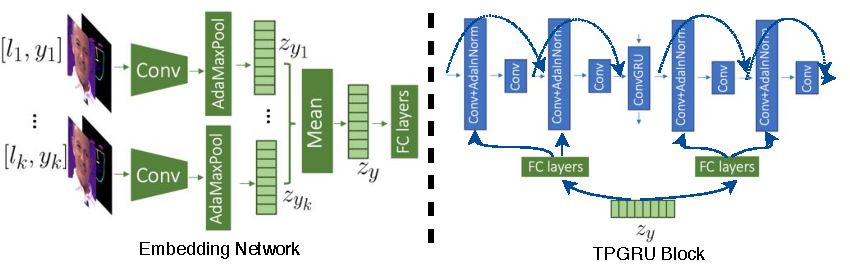
\includegraphics[width=1.0 \linewidth]{latex/images/network_details_reduce.pdf}
\caption{Detailed structure of the embedding network and the \textit{TP-GRU} block.}
% \vspace{-6.5mm}
\label{fig:network_details}
\end{figure}
\noindent {\bf{TP-GRU}}\indent The appearance latent vector $\mathbi{z}_y$ computed from the embedding network contains the global texture information of target identity. At each time step $t$, after encoding the input pair $[\mathbi{l}_t, \tilde{\mathbi{y}}_{t}]$, the resultant feature $\mathbi{e}_t$ carries the detailed facial expression and geometry information. Rather than simply concatenating the feature vectors~\cite{chung2017you,zhou2019talking,chen2018lip,chen2019hierarchical,ijcai2019-129}, we propose a \textit{TP-GRU} module, which aims to fuse appearance feature, geometry feature and expression feature in a recurrent manner. The \textit{TP-GRU} (see right part in Fig.~\ref{fig:network_details}) consists of eight convolution layers with residual connections and one layer of convolutional GRU. There are four convolution layers normalized by adaptive instance normalization (AdaIN)~\cite{huang2017arbitrary}. The AdaIN layers are initialized with zero means and unit variance at each time step. We then adaptively compute two sets of affine transformation parameters $[\boldsymbol{\mu},\boldsymbol{\sigma}^2]_1, [\boldsymbol{\mu},\boldsymbol{\sigma}^2]_2$ using $\mathbi{z}_y$ via two separately-learnable fully connected perceptions. We apply the two sets of parameters as scalars and biases to scale the activations in the two AdaIN layers before and after GRU, respectively. The intuition is that the affine transformation is spatially invariant and hence we can inject global appearance information to \textit{TP-GRU}. We empirically show TP-GRU learn to fuse novel appearance and strongly generalize to novel identities with different poses, appearances, and expressions (see Tab.~\ref{tab:lmark_tb} CSIM score). 


\subsection{Attention-based Builder} 
\label{subsec:AttBuilder}
After the \textit{TP-GRU} module, the frame feature $\mathbi{e}_t$ is up-sampled by several convolutional blocks with an up-sampling layer. Similar to~\cite{pumarola2019ganimation}, we apply convolution with sigmoid and hyperbolic tangent activation functions on the up-sampled image feature to get texture attention map $\boldsymbol{\alpha}_t \in \mathbb{R}^{H\times W \times1}$ and synchronized facial motion map $\mathbi{m}_t \in \mathbb{R}^{H\times W \times C}$, respectively. As mentioned before, our animation frame $\tilde{\mathbi{y}}_t$ also contains valuable texture information with better alignment to the ground-truth $ \mathbi{y}_t  $. Thus the foreground of the image $f_t \in \mathbb{R}^{H\times W \times C}$ at time step $t$ is governed by the combination:
\begin{equation}
\begin{aligned}
 f_t =   \boldsymbol{\alpha}_t \odot \mathbi{m}_t + (\mathbf{1}- \boldsymbol{\alpha}_t ) \odot \tilde{\mathbi{y}}_t  \enspace,
\end{aligned}
\label{eq:foreground}    
\end{equation}
where the $\odot$ is element-wise multiplication. Note that compared to previous methods~\cite{pumarola2019ganimation,chen2019hierarchical,wang2018high}, which use a reference image rather than $\tilde{\mathbi{y}}_t$, our combination method is much better in talking-head video generation task especially when there is large head motion between reference frames and the ground-truth frame. Furthermore, in our empirical study, this composition can correct the identity mismatch in the generation stage and make the network converge faster. 

We observe that the background of target image $\mathbi{y}_t$ at step $t$ is expected to be, on average, more visually similar to image that contains head with similar pose in a video recorded by still camera. The combination of foreground $f_t$ and background $\mathbi{y}_t^s$ follows the similar protocol in Eq.~\ref{eq:foreground}. We apply a Foreground-Attention (FG-Att) on $\mathbi{y}_t^s$, $ \tilde{\mathbi{y}}_t$ and the frame feature $\mathbi{e}_t$ to obtain the foreground attention. Specifically, we concatenate  $\mathbi{y}_t^s$ and $\tilde{\mathbi{y}}_t$ in channel-wise to $[\mathbi{y}_t^s, \tilde{\mathbi{y}}_t] \in \mathbb{R}^{H\times W \times 2C}$ and apply three convolutional layers on it to have a prior foreground feature $\mathbi{p}_t \in \mathbb{R}^{H\times W \times 64}$ and concatenate with the frame feature $\mathbi{e}_t$ in channel wise to have $[\mathbi{p}_t, \mathbi{e}_t] \in \mathbb{R}^{H\times W \times 128}$. Then we feed the concatenated feature to one convolution layer with sigmoid activation function to compute an adaptively learned foreground attention map $\boldsymbol{\beta}_t \in \mathbb{R}^{H\times W \times 1}$. With this foreground attention map, dilated background image $\mathbi{y}_t^s$ and computed foreground $f_t$, the final image frame is obtained by:
\begin{equation}
\begin{aligned}
 \hat{y}_t =   \boldsymbol{\beta}_t \odot f_t + (\mathbf{1}- \boldsymbol{\beta}_t ) \odot\mathbi{y}_t^s  \enspace.
\end{aligned}
\label{eq:background}    
\end{equation}
We apply dilation operation on $\mathbi{y}_t^s$ to alleviate the misalignment issue caused by $c_t$ in the motion matching step. We also tried to learn an optic flow from $[f_t, \mathbi{y}_t^s ]$ to warp $\mathbi{y}_t^s$ to fix the misalignment issue, but the results show that dilation is more efficient and accurate (see Tab.~\ref{tab:alation}).
 
\subsection{Objective Function}
\label{subsec:loss}

The Multi-Scale Discriminators~\cite{wang2018high} are employed to differentiate the real and synthesized video frames. We use two discriminators that have the same network structure but operate at two different image scales. At each time step $t$, we downsample the pair of image frame and associated converted landmark image $[\mathbi{l}_{t}, \mathbi{y}_{t}] \in \mathbb{R}^{H\times W \times 2C} $ by a factor of 2 to create an pyramid of two scales. The discriminators $D_1$ and $D_2$ are trained on the two input scales, respectively. Thus, the best sequential generator $G^*$ is found by solving the following optimization problem:
\begin{equation}
\begin{aligned}
& G^* = \argminA_G\bigg{(} \Big{(} \max_{D_1,D_2}\sum_{k=1,2} \mathcal{L}_{\text{GAN}}(G,D_k) \\
& + \lambda_{\text{FM}} \sum_{k=1,2} \mathcal{L}_{\text{FM}}(G,D_k) \Big{)} + \lambda_{\text{PCT}} \mathcal{L}_{\text{PCT}}(G)\bigg{)}  \enspace,
\end{aligned}
\label{eq:loss}    
\end{equation}
where $\mathcal{L}_{\text{GAN}}$ is the LSGAN loss~\cite{mao2017least}, $\mathcal{L}_{\text{FM}}$ is the feature matching loss proposed in 
~\cite{wang2018high} to stabilize the training. The $\mathcal{L}_{\text{PCT}}$ is the perceptual loss term, which measures the perceptual similarity distance between the ground truth video frames and the synthesized video frames. The $\lambda_{\text{FM}}$ and $\lambda_{\text{PCT}}$ control the importance of three loss terms. 

The perceptual loss~\cite{johnson2016perceptual} term $\mathcal{L}_{\text{PCT}}$ in Eq.~\ref{eq:loss} regularizes the training in two different perceptual respects: we employ the VGG19~\cite{Simonyan15} feature extractor pretrained on ImageNet~\cite{deng2009imagenet} classification to increase the sharpness of synthesized video. The VGGFace~\cite{parkhi2015deep} feature extractor pretrained on the VGG-Face dataset is employed to consider the identity similarities between synthesized videos and ground truth videos.  


\section{Talking-head Generation with rhythmic head motion }
\label{sec:infer}

% \CXu{This section tells about inference with different strategies, or aka driving modalities.}

During training (see Sec.~\ref{sec:method}), we generate videos based on ground truth landmarks $\mathbi{l}_{\tau+1:T}$ in order to supervise the training. In other word, we use ground truth head motion $\mathbi{h}_{\tau+1:T}$ and ground truth facial expression $\hat{\mathbi{l}}_{\tau+1:T}$ to synthesize videos. At the inference stage, the facial expression $\hat{\mathbi{l}}_{\tau+1:T}$ can be transferred from user input data ${\mathbi{x}}_{\tau+1:T}$ (e.g., audio signal, landmarks and RGB frames). And the head movement ${\mathbi{h}}_{\tau+1:T}$ can be inferred either from conditioned videos or the 3-second video ${\mathbi{y}}_{1:\tau}$ of the target subject. Here, we mainly discuss such a novel protocol: we generate $\hat{\mathbi{l}}_{\tau+1:T}$ from an arbitrary speech signal, and infer $\hat{\mathbi{h}}_{\tau+1:T}$  from the input short video ${\mathbi{y}}_{1:\tau}$. So the Eq.~\ref{eq:training} can be rewritten as:
\begin{equation}
\begin{aligned}
\hat{\mathbi{y}}_{ \tau+1:T} =  F( \mathbi{y}_{1:\tau},\hat{\mathbi{l}}_{\tau+1:T}   \circledast \hat{\mathbi{h}}_{\tau+1:T} )  \enspace,
\end{aligned}
\label{eq:inference}    
\end{equation}
where the $\circledast$ is the inverse operator of motion disentangler in Sec.~\ref{subsec:3d_man} and $\hat{\mathbi{h}}_{\tau+1:T}$ can be approximated in Sec.~\ref{subsec:movement}.
%
%our model can generate video based on an arbitrary audio signal or an arbitrary video/landmark sequence. We transfer the input audio signal/video sequence to facial landmarks and use \textit{motion disentangler} to disentangle the facial expression $\hat{\mathbi{l}}_{\tau+1:T}$, which only contains facial-expression-correlated information. Then we use the head motion extrapolation module to extrapolate the individual head movements $\hat{\mathbi{h}}_{\tau+1:T}$ using the input reference video. Next, based on the extrapolated head motion $\hat{\mathbi{h}}_{\tau+1:T}$ and 3D mesh $\mathcal{M}$, our projector outputs corresponding 3D projection $\tilde{\mathbi{y}}_{\tau+1:T}$. Then we feed the manipulated facial landmark with corresponding 3D animation $[\hat{\mathbi{l}}_{\tau+1:T}  \circledast \hat{\mathbi{h}}_{\tau+1:T}, \tilde{\mathbi{y}}_{\tau+1:T} ] $ to the framework to get the synthesized video sequence $\hat{\mathbi{y}}_{\tau+1:T}$. 
The facial expressions are controlled by $\hat{\mathbi{l}}_{\tau+1:T}$ and the $\hat{\mathbi{h}}_{\tau+1:T}$ carries the natural head motion. 
 
 
\begin{figure}
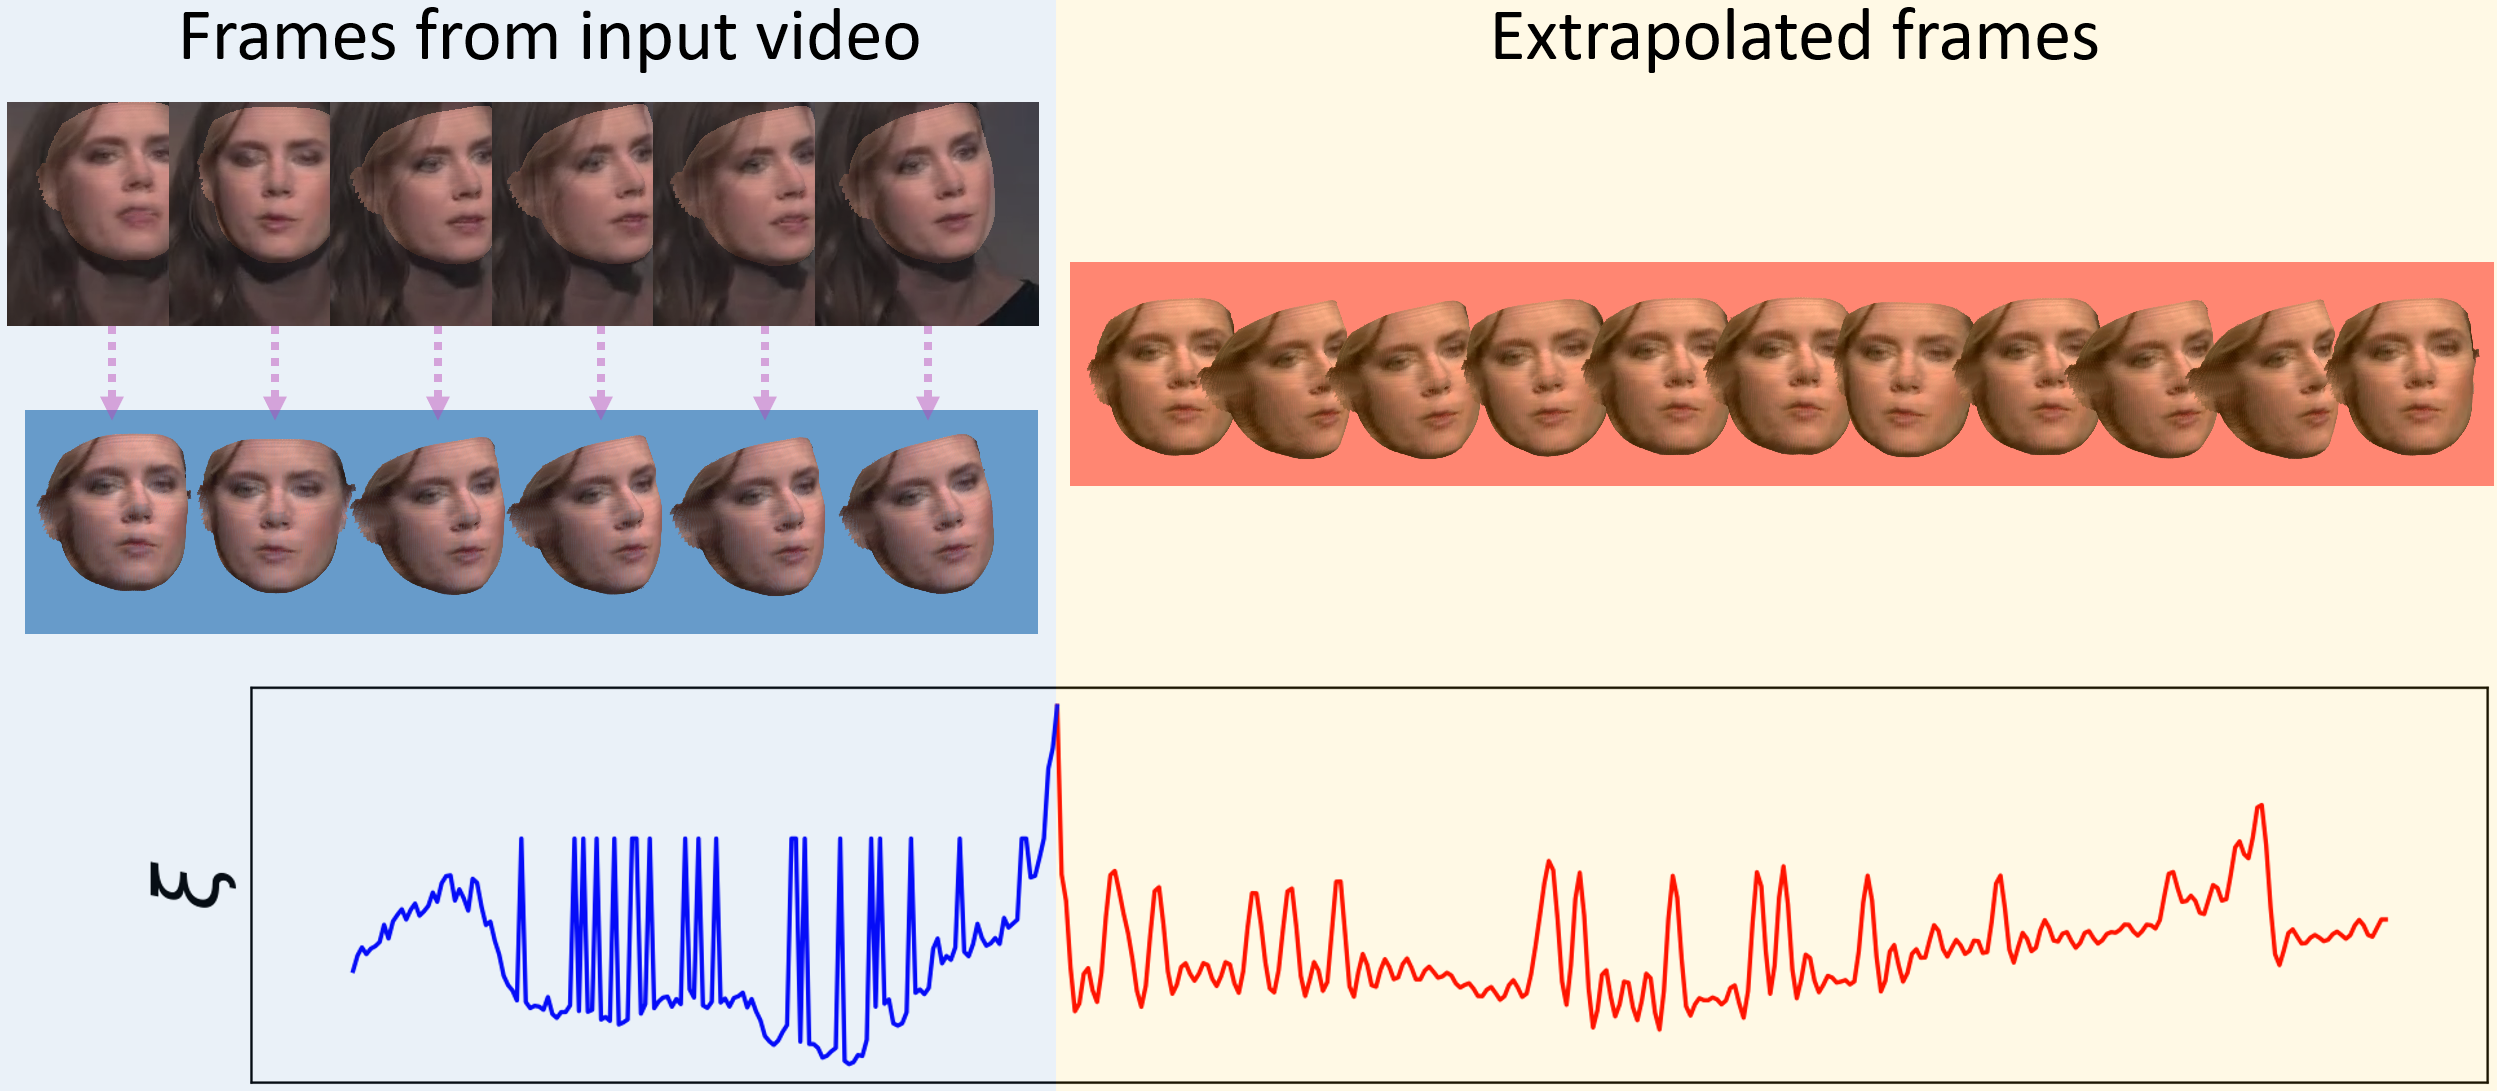
\includegraphics[width=1.0 \linewidth]{latex/images/faces.png}
%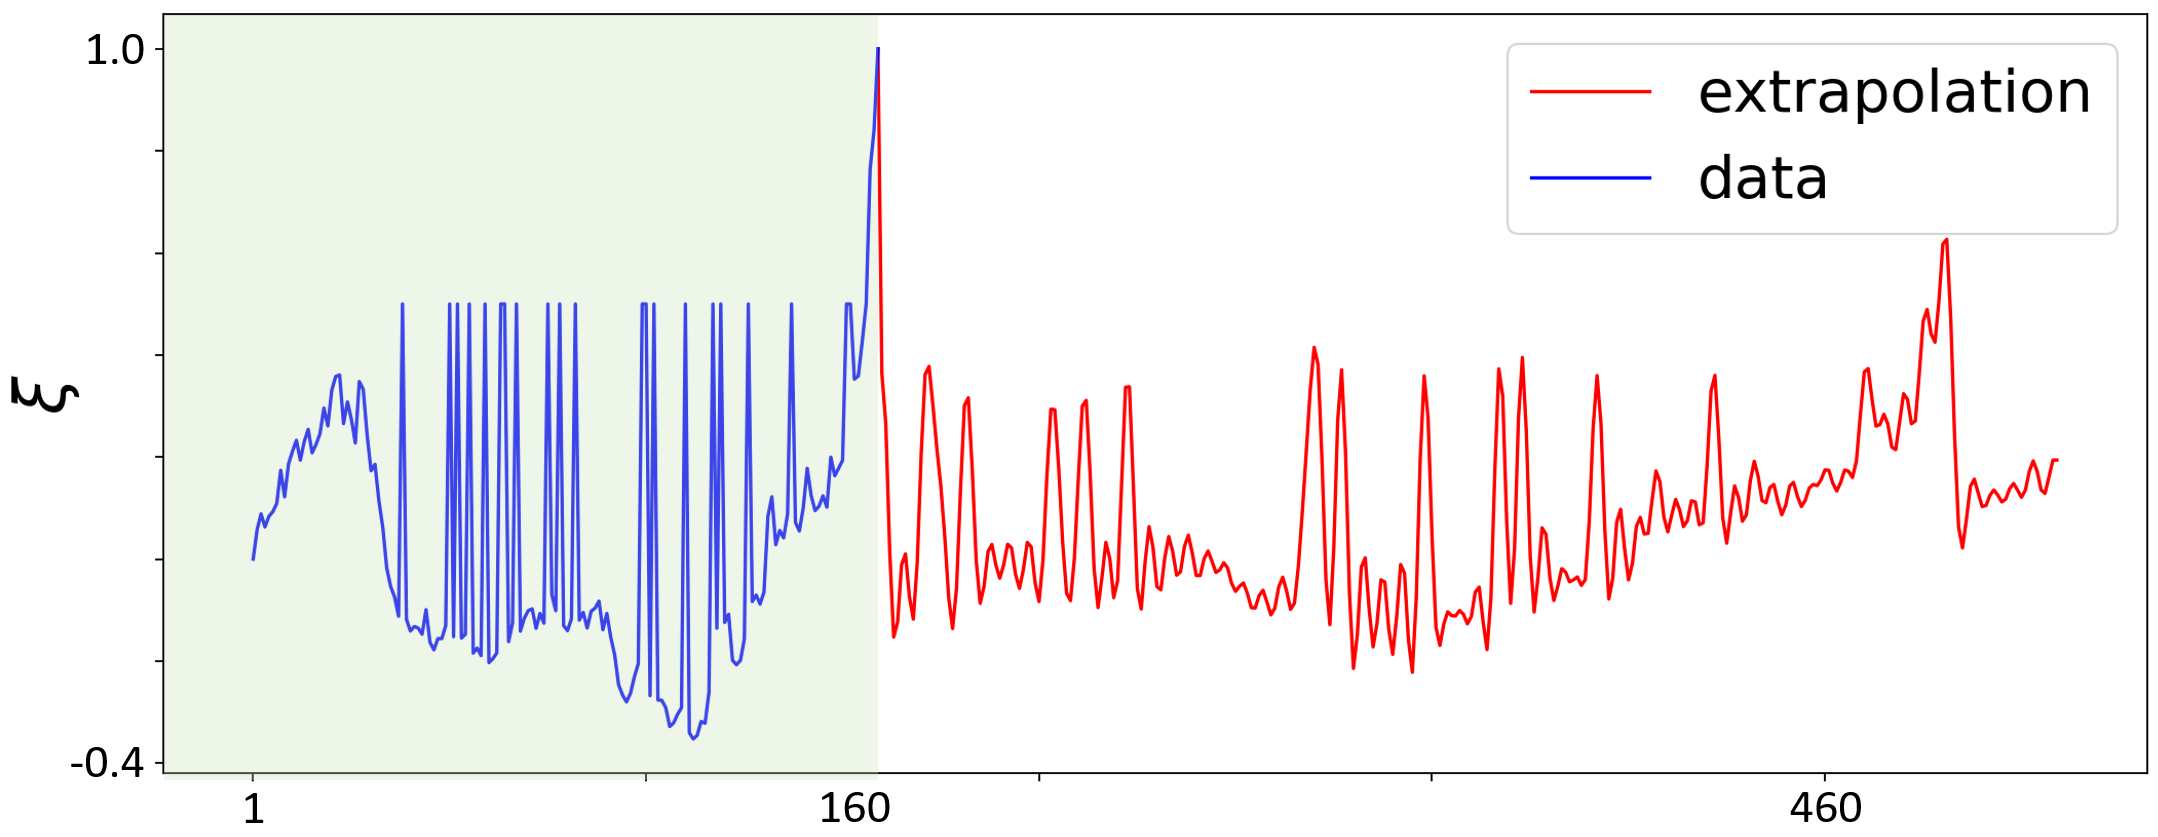
\includegraphics[width=1.0 \linewidth]{latex/images/rtextra/curve.png}
% 
\includegraphics[width=1.0 \linewidth]{latex/images/rtextra/tet.png}
\caption{Extrapolate head motion from input frames. For the left column: the first row is the sequence of input frames, the second row is the visualization of head motion for each input frame by applying the correspondence $[\mathbf{R},\mathbf{T}]$ to the reconstructed 3D face, and the third row is the parameterized motion $\xi_{1:\tau}$ for input frames. For the right column: the first row is the extrapolated frames of head motion visualization, and the second row is the extrapolated motion parameterization $\xi_{\tau+1:T}$.}
\label{fig:rtextra}
\end{figure}
 
%%%%%%%%%%%%%%%%%%%%%%%%%%
\begin{table*}[t]
    \centering
  \begin{tabular*}{0.7\linewidth}{  p{1.9cm} p{1.0cm} p{1.0cm} p{1.0cm}|p{1.0cm} p{1.0cm} p{1.0cm} }
      \toprule
      \toprule
Method & \multicolumn{6}{c}{Audio-driven}   \\ \hline

Dataset & \multicolumn{3}{c}{LRW} & \multicolumn{3}{c}{VoxCeleb2}   \\
      \midrule
& {LMD$\downarrow$} & {CSIM$\uparrow$} & {FID$\downarrow$} & {LMD$\downarrow$} & {CSIM$\uparrow$} & {FID$\downarrow$}  \\

\hline
{X2Face~\cite{wiles2018x2face}} & 1.60& 0.21& 56.4 & 2.35  & 0.19  & 59.1\\
 \hline
 {S2V~\cite{chung2017you}}& 1.63 & 0.35 & 56.8 & 2.01  & 0.33  & 64.2    \\ \hline

 {ATVGnet~\cite{chen2019hierarchical}}  & 1.37 & 0.31 & 58.0  &1.77  & 0.34 & 60.3 \\    \hline
  {CRVG~\cite{ijcai2019-129}}  & \textbf{1.29} & 0.36 & 44.4 & \textbf{1.59}   & 0.31 & 47.6 \\    \hline

  {DAVS~\cite{zhou2019talking}}  & 1.55 & 0.29 & 49.5 & 1.80   & 0.27  & 51.1\\    \hline
    \bottomrule
  { Ours } & 1.31  & \textbf{0.47 }& \textbf{29.7}& 1.84  &\textbf{0.42 } &\textbf{35.8 }\\ \hline
      \bottomrule
  \end{tabular*}
  \caption{Quantitative results of different audio to video methods on LRW dataset and VoxCeleb2 dataset. Our model mentioned in this table are trained from scratch. We bold each leading score.}
    \label{tab:audio_tb}
\end{table*}
%%%%%%%%%%%%%%%%%%%%%%%%%
%%%%%%%%%%%%%%%%%%%%%%%%%%

\begin{table*}[h]
    % \centering
    \begin{center}
    \begin{tabular*}{0.75\linewidth}{  l | c c c | c c c}
%   \begin{tabular*}{0.7\linewidth}{  p{2.8cm}| p{0.9cm} p{0.9cm} p{1.2cm} |p{1.2cm} p{0.9cm} p{0.9cm}}
      \toprule
      \toprule
 Method & \multicolumn{6}{c}{Landmark-driven}   \\ \hline

Dataset & \multicolumn{3}{c}{VoxCeleb1} & \multicolumn{3}{c}{VoxCeleb2}  \\
      \midrule
&{CSIM$\uparrow$}& {SSIM$\uparrow$}&{FID$\downarrow$} &{CSIM$\uparrow$}& {SSIM$\uparrow$}&{FID$\downarrow$}  \\
\hline  
{X2Face~\cite{wiles2018x2face}-1} &0.16 &0.68 &45.8 & 0.19  & 0.65 & 49.4 \\ \hline

 {ATVGnet~\cite{chen2019hierarchical}-1}&0.11 & 0.66 & \textbf{37.9} & 0.14 & 0.68 & 42.2  \\    \hline

 {pix2pixHD~\cite{wang2018high}-1} & { 0.09 } &{ 0.56} &{ 42.7} & { 0.11 } &{ 0.52} &{ 43.9} \\ \hline
 {FSVid~\cite{zakharov2019few}-1} & {0.15 } &{0.67  } &{ 43.0} & 0.21 & 0.64 & 41.2   \\ \hline
%   {FSvid2vid-1} & { } &{ } &{ } & & &  & {} &{} &{} &{}&{}&{}   \\ \hline
 {Ours-1} &\bf{0.22} & \bf{0.70} &{40.5} & \bf{0.27 } & \bf{ 0.68} &\bf{34.9 }  \\ \hline
 \bottomrule
{X2Face~\cite{wiles2018x2face}-8} &0.17 &0.73 &51.5 & 0.21  & 0.67 & 56.8 \\ \hline
 {pix2pixHD~\cite{wang2018high}-8} & { 0.12} &{ 0.64} &\bf{ 35.1} &{0.14}&{0.66}&{37.2} \\ \hline 
 {FSVid~\cite{zakharov2019few}-8} & {0.17} &{0.71} &{38.0} & {0.21}&\bf{0.69}&{36.1}  \\ \hline
 {Ours-8} &\bf{0.31} & \bf{0.74} &{39.5} & {\bf{0.35}} &{{0.68}} &\bf{30.1}  \\ \hline
  \bottomrule 
{X2Face~\cite{wiles2018x2face}-32} & 0.18&0.75 & 56.5 & 0.27  & 0.71  & 44.9 \\ \hline
 {pix2pixHD~\cite{wang2018high}-32} & {0.16} &{0.70} &{\textbf{24.0}} &{0.20}&{0.68}&{35.7}  \\ \hline
 {FSVid~\cite{zakharov2019few}-32} & {0.19} &{0.73 } &{29.5} & {0.28}&\bf{0.72}&{34.9}   \\ \hline
 {Ours-32} &\bf{0.39} & \bf{0.76} &{33.8} & \bf{0.40} &{0.69} &\bf{28.4} \\ \hline
      \bottomrule
  \end{tabular*}
  \end{center}
  \caption{Quantitative results of different landmark to video methods on VoxCeleb1 dataset and VoxCeleb2 dataset. Our model mentioned in this table are trained from scratch. We bold each leading score. The number after each method denotes the $K$ frames of the target subject.}
    \label{tab:lmark_tb}
\end{table*}

\subsection{The natural head motion extrapolation}
\label{subsec:movement}

To synthesize realistic talking-head videos, we introduce a head motion extrapolation method, which predicts the head movements $\hat{\mathbi{h}}_{\tau +1:T}$ based on the 3D landmarks $\mathbi{l}_{1:\tau}$ computed from ${\mathbi{y}}_{1:\tau}$. Thanks to the Lie Group framework for affine interpolation~\cite{bansal2019affine}, from two given affine transformations $\mathbb{T}_1$ and $\mathbb{T}_2$, an intermediate transformation can be represented as a $\mathbb{T}(\xi), \xi\in[0,1]$, such that $\mathbb{T}(0)=\mathbb{T}_1$ and $\mathbb{T}(1)=\mathbb{T}_2$. Specifically, for rigid transformation, the Lie group representation of the interpolated transformation between $[\mathbf{R},\mathbf{T}]_1$ and $[\mathbf{R},\mathbf{T}]_\tau$ at $\xi$, is given by:
\begin{equation}
\label{eqn:rtextra}
[\mathbf{R},\mathbf{T}](\xi) = [\mathbf{R},\mathbf{T}]_1 \exp\left(\xi \log\left([\mathbf{R},\mathbf{T}]_1^{-1}[\mathbf{R},\mathbf{T}]_\tau\right)\right).
\end{equation}
Closed-form expressions of the exponential and log maps can be found in~\cite{bansal2019affine}.
Therefore, $[\mathbf{R},\mathbf{T}]_{1:\tau}$ can be mapped to the parameter space $\xi_{1:\tau}=\{\xi_1,\xi_2,...,\xi_\tau\}$, such that $[\mathbf{R},\mathbf{T}](\xi_i)\approx [\mathbf{R},\mathbf{T}]_i$. Note that $\xi_1=0$, $\xi_\tau=1$ and $\xi_i (1<i<\tau)$ can be obtained by solving 
$\underset{x}{\text{argmin}} \begin{Vmatrix}[\mathbf{R},\mathbf{T}](\xi_i) - [\mathbf{R},\mathbf{T}]_i\end{Vmatrix}_F$.
We observed that the movement of a talking-head is bounded and has some periodic trend. Hence, we apply the Discrete Fourier Transformation on $\xi_i^\tau$ and choose the first $45$ harmonics to construct the Fourier series $\mathcal{F}(\cdot)$, such that $\mathcal{F}(i)\approx \xi_i, i\in[1,\tau]$. Then we can extrapolate $\xi_{\tau+1:T}$ by $\{\mathcal{F}(\tau+1),...,\mathcal{F}(T)\}$. Finally, applying  Eq.~\ref{eqn:rtextra} on $\xi_{\tau+1:T}$ will result to $[\hat{\mathbf{R}},\hat{\mathbf{T}]}_{\tau + 1:T}$.
In Fig.~\ref{fig:rtextra}, we visualize the head motion by applying $[\mathbf{R},\mathbf{T}]_i$ to the reconstructed 3D face $\mathcal{M}$ and then rendering with the 3D Projector (see Sec.~\ref{subsec:3d_man}). The bottom curve in Fig.~\ref{fig:rtextra} is the parameter $\xi$ over time.


\section{Experiments}
\label{sec:experiments}
In this section, we conduct thoughtful experiments to demonstrate the effectiveness of the proposed architecture for video generation. 
%Sec. 4.1 explains datasets and implementation in detail. Sec. 4.2 shows our results along with other state-of-the-art methods. We show user studies and ablation study in Sec.4.3 and Sec. 4.4 respectively.

\subsection{Experimental Setup}
\label{subsec:exp_setup}

\noindent \textbf{Dataset} \quad We quantitatively and qualitatively evaluate our approach on three datasets with talking-head videos: VoxCeleb2~\cite{Chung18b} (224p videos at 25 FPS), LRW~\cite{Chung16} (256p videos at 29 FPS), and VoxCeleb1~\cite{Nagrani17} (256p videos at 1 FPS). The VoxCeleb2 contains over 1 million utterances for 6,112 celebrities, extracted from videos uploaded to YouTube. We follow the same train-test split as in \cite{Chung18b}. The LRW dataset consists of 500 different words spoken by hundreds of different speakers in the wild. VoxCeleb1 contains much fewer videos comparing to VoxCeleb2, thus we only use the testing set to test our approach. 

\noindent \textbf{Implementation Details} \quad We follow the training procedure from \cite{chen2019hierarchical}. We adopt ADAM~\cite{KingmaB14} optimizer with $\text{lr} = 2 \times 10^{-4}$ and $(\beta_1,\beta_2) = (0.5,0.999)$. During training, the length of TP-GRU in image translator is 16, and we select $K = 1,8,32$ in our embedding network. The $\tau$ in all experiments is 64. The $\lambda_{\text{FM}} = 10$ and $\lambda_{\text{PCT}} = 1$ in Eq.~\ref{eq:loss}.  
%All experiments are conducted on an NVIDIA DGX-1 machine with 8 32GB V100 GPUs. 
   
\subsection{Results and Analysis}
\label{subsec:quanti_res}
\noindent \textbf{Evaluation Metrics} \quad We use several criteria for quantitative evaluation. We use Fréchet Inception Distance (FID)~\cite{heusel2017gans}, mostly quantifying the fidelity of synthesized images, structured similarity (SSIM)~\cite{wang2004image}, commonly used to measure the low-level similarity between the real images and generated images. To evaluate the identity preserving ability, we use cosine similarity (CSIM) used in \cite{zakharov2019few}, which computes the cosine similarity between embedding vectors of the state-of-the-art face recognition network~\cite{deng2019arcface} for measuring identity mismatch. To evaluate whether the synthesized video contains accurate lip movements that correspond to the input condition, we adopt the evaluation matrix Landmarks Distance (LMD) proposed in~\cite{chen2018lip}.


\begin{figure}
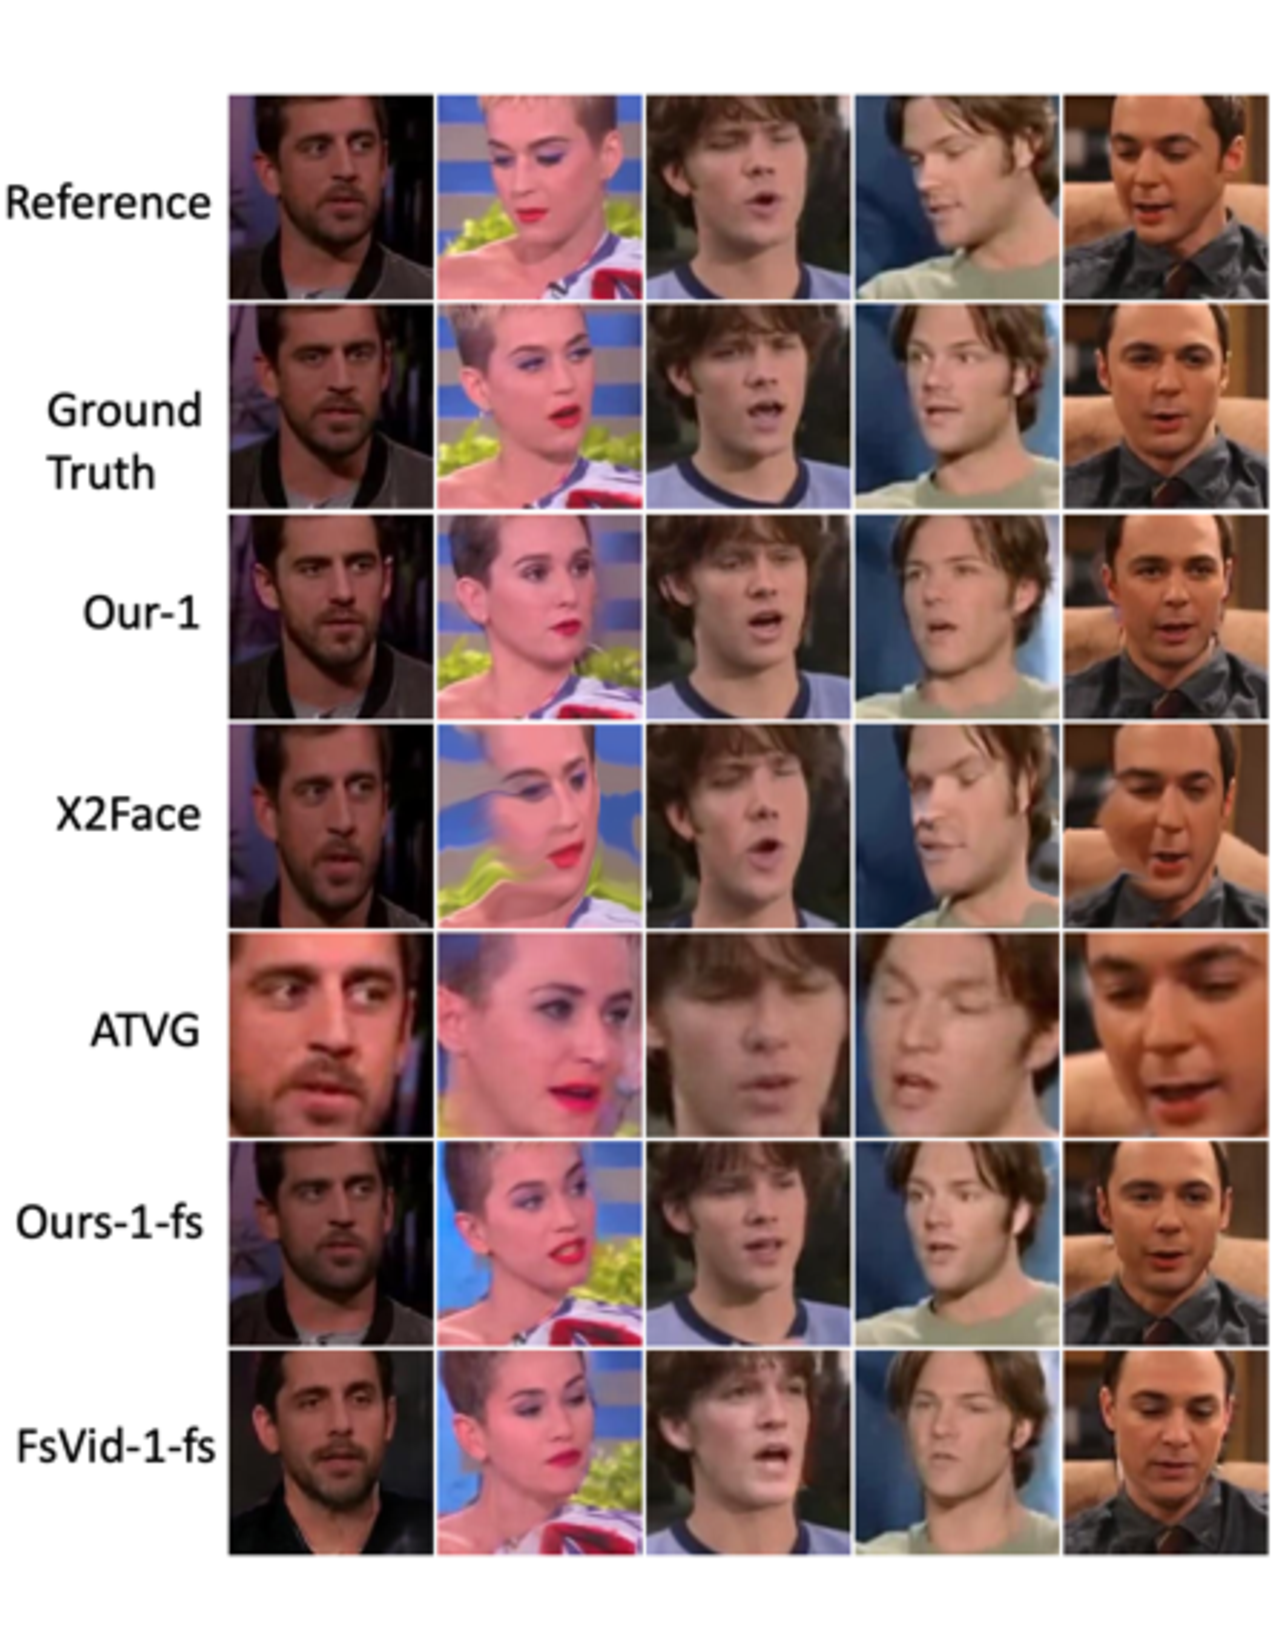
\includegraphics[width=0.95 \linewidth]{latex/images/compare1_reduce.pdf}
\caption{The qualitative results of different landmark/image-driven methods on VoxCeleb2 testing set. The third to fifth rows are zero-shot results. The last two rows are one-shot results.}
% \vspace{-6.5mm}
\label{fig:compare1}
\end{figure}


\noindent \textbf{Comparison with Other Methods} \quad We compared our method with two sets of state-of-the-art methods. We first compare our approach with those audio to video generation methods: ATVGnet~\cite{chen2019hierarchical}, X2Face~\cite{wiles2018x2face}, S2V~\cite{chung2017you}, and DAVS~\cite{zhou2019talking}, which take audio and one frame as inputs and synthesize a talking face saying the speech. We show the results in Tab.~\ref{tab:audio_tb}.
We also compare our approach with state-of-the-art landmark-to-video generation methods: X2Face~\cite{wiles2018x2face}, ATVGnet~\cite{chen2019hierarchical}, pix2pixHD~\cite{wang2018high}, FSVid\cite{zakharov2019few} on VoxCeleb1 and VoxCeleb2 datasets. According to Tab.~\ref{tab:lmark_tb}, our approach achieves best performance in most of the evaluation matrices. It is worth to mention that our method outperforms other methods in terms of the CSIM score, which demonstrates the generalizability of our method. We choose different $K$ here to better understand our matching scheme. We can see that with larger $K$ value, the inception performance (FID and SSIM) improve dramatically. 

To further explore the upper-bound of our approach, we also train our model in the same few-shot setting described in their papers to do the comparison. Note that we only select $K$ images from the first 64 frames, and other comparing methods select $K$ images from the whole video sequence, which arguably gives other methods an advantage.


%%%%%%%%%%%%%%%%%%%%%%%%%%%%%%%%%%%%%%%%
% \begin{table}[t]
%     \centering
%   \begin{tabular*}{0.45\linewidth}{  p{2.2cm} | p{0.95cm} p{0.9cm} p{0.9cm}}
%       \toprule
%       \toprule
% Method & \multicolumn{2}{c}{Few-shot learning}   \\ \hline
%       \midrule
% & {CSIM$\uparrow$} &{SSIM$\uparrow$}&{FID$\downarrow$}  \\ \hline
% {FSvid2vid-1} & 0.35 & 0.64 & 46.1 \\ \hline
% {Our-1} & \bf{0.47}  & \bf{0.64}  & \bf{30.3}  \\
%     \bottomrule
% {FSvid2vid-8} & 0.42 & 0.68 & 42.2 \\ \hline
% {Our-8} & \bf{0.58}  & \bf{0.73}   & \bf{26.5}  \\ 
%     \bottomrule
% {FSvid2vid-32} & 0.45 & 0.72 & 30.6 \\ \hline
% {Our-32} & \bf{0.61} &\bf{ 0.72} & \bf{26.1}  \\ \hline
%     \bottomrule
%   \end{tabular*}
%   \caption{Quantitative results of few-shot learning on VoxCeleb2 dataset. For fair comparison, here we remove the recurrent unit in our model. We bold each leading score.}
%     \label{tab:few-shot_tb}
% \end{table}
%%%%%%%%%%%%%%%%%%%%%%%%%

\begin{table}[ht]
\begin{minipage}[b]{0.45\linewidth}\centering
\begin{tabular}{  p{2.0cm} | p{0.95cm} p{0.8cm} p{0.9cm}}
      \toprule
      \toprule
Method & \multicolumn{2}{c}{Few-shot learning}   \\ \hline
      \midrule
& {CSIM$\uparrow$} &{SSIM$\uparrow$}&{FID$\downarrow$}  \\ \hline
{FSvid2vid-1} & 0.35 & 0.64 & 46.1 \\ \hline
{Our-1} & \bf{0.47}  & \bf{0.64}  & \bf{30.3}  \\
    \bottomrule
{FSvid2vid-8} & 0.42 & 0.68 & 42.2 \\ \hline
{Our-8} & \bf{0.58}  & \bf{0.73}   & \bf{26.5}  \\ 
    \bottomrule
{FSvid2vid-32} & 0.45 & 0.72 & 30.6 \\ \hline
{Our-32} & \bf{0.61} &\bf{ 0.72} & \bf{26.1}  \\ \hline
    \bottomrule
  \end{tabular}
  \caption{Quantitative results of few-shot learning on VoxCeleb2 dataset. For fair comparison, here we remove the recurrent unit in our model. We bold each leading score.}
    \label{tab:few-shot_tb}
\end{minipage}
\hspace{0.5cm}
\begin{minipage}[b]{0.45\linewidth}
\centering
\begin{tabular}{  p{3.2cm} | p{0.9cm} p{0.9cm} p{0.9cm}}
      \toprule
      \midrule
Method & {CSIM$\uparrow$} &{SSIM$\uparrow$}&{FID$\downarrow$}  \\ \hline
{w/o \textit{TP-GRU}-1} & \textbf{0.30} & 0.66 &\bf{33.8}  \\ \hline
{with warping-1} & 0.21 & 0.64 & 39.1 \\ \hline
{w/o \textit{Motion Matcher}-1}  & 0.22 & 0.64 & 78.5 \\ \hline
{Our-1} & {0.27} & \bf{0.68} &  {34.9} \\
    \bottomrule
{w/o \textit{TP-GRU}-8} &0.32  & 0.67 & 36.6  \\ \hline
{with warping-8} & 0.29 & 0.62 & 37.4 \\ \hline
{w/o \textit{Motion Matcher}-8} & 0.27 & 0.65 & 59.4 \\ \hline

{Our-8} & \textbf{0.35} & \textbf{0.68} &  \textbf{30.1}\\
    \bottomrule
{w/o \textit{TP-GRU}-32} & 0.34 &\textbf{ 0.70} & 34.0 \\ \hline
{with warping-8} & 0.28 & 0.65 & 37.4 \\ \hline
{w/o \textit{Motion Matcher}-32} &  0.26& 0.66 & 52.6 \\ \hline

{Our-32} & \bf{0.40}  & {0.69} &  \textbf{28.4}   \\
    \bottomrule
  \end{tabular}
  \caption{Ablation studies on VoxCeleb2 dataset. Our model mentioned in this table are trained from scratch. We bold each leading score.}
    \label{tab:alation}
\end{minipage}
\end{table}

%%%%%%%%%%%%%%%%%%%%%%%%%%%%%%%%%%%%%%%%
% \begin{table}[t]
%     \centering
%   \begin{tabular*}{0.6\linewidth}{  p{3.8cm} | p{0.9cm} p{0.9cm} p{0.9cm}}
%       \toprule
%       \midrule
% Method & {CSIM$\uparrow$} &{SSIM$\uparrow$}&{FID$\downarrow$}  \\ \hline
% {w/o \textit{TP-GRU}-1} & \textbf{0.30} & 0.66 &\bf{33.8}  \\ \hline
% {with warping-1} & 0.21 & 0.64 & 39.1 \\ \hline
% {w/o \textit{Motion Matcher}-1}  & 0.22 & 0.64 & 78.5 \\ \hline
% {Our-1} & {0.27} & \bf{0.68} &  {34.9} \\
%     \bottomrule
% {w/o \textit{TP-GRU}-8} &0.32  & 0.67 & 36.6  \\ \hline
% {with warping-8} & 0.29 & 0.62 & 37.4 \\ \hline
% {w/o \textit{Motion Matcher}-8} & 0.27 & 0.65 & 59.4 \\ \hline

% {Our-8} & \textbf{0.35} & \textbf{0.68} &  \textbf{30.1}\\
%     \bottomrule
% {w/o \textit{TP-GRU}-32} & 0.34 &\textbf{ 0.70} & 34.0 \\ \hline
% {with warping-8} & 0.28 & 0.65 & 37.4 \\ \hline
% {w/o \textit{Motion Matcher}-32} &  0.26& 0.66 & 52.6 \\ \hline

% {Our-32} & \bf{0.40}  & {0.69} &  \textbf{28.4}   \\
%     \bottomrule
%   \end{tabular*}
%   \caption{Ablation studies on VoxCeleb2 dataset. Our model mentioned in this table are trained from scratch. We bold each leading score.}
%     \label{tab:alation}
% \end{table}
%%%%%%%%%%%%%%%%%%%%%%%%%
\noindent \textbf{Ablation Studies} \quad We conduct thoughtful ablation experiments to study the contributions of each module we introduced in Sec.~\ref{sec:method}. The ablation studies are conducted on VoxCeleb2 dataset. We train and test our model with different $K$ values.
As shown in Tab.~\ref{tab:alation}, each component contributes to the full model. We can find that the \textit{Motion Matcher} is critical to our full model. We attribute it to the better ability of generating smooth transactions between adjacent frames. We also replace the dilation operation with warping to fix the $c_t$ caused by \textit{Motion Matcher} and we can find that with warping, the performance drops. We attribute it to the poor ability of optic follow on complicated dynamics in head movements (e.g., head rotation). Also, we can find that with more reference images (larger $K$ value), our model achieves better performance. We attribute it to the lower $c_t$ since we have more choices to match the target frame. 

\noindent \textbf{Qualitative Results} \quad We show our qualitative comparison in Fig.~\ref{fig:compare1} with other state-of-the-art methods. We can find that our approach can generate correct head motion and facial expressions, while preserving the appearance information. We show more audio-driven video results and interesting manipulations on head motion and facial expressions in \textit{Supplementary Material}   please refer to the video and images in the \textit{Supplementary Material}.

\section{Conclusion and Discussion}
In this paper, we propose a novel approach to model the head motion and facial expression explicitly, which can synthesize talking-head videos with rhythmic head motion of unseen subjects at the inference time. By leveraging the 3D manipulation, our model can generate talking-head videos with controllable head motion and facial expressions. Experimental results showed that our method performs favorably against the competing methods.
  

\clearpage
% ---- Bibliography ----
%
% BibTeX users should specify bibliography style 'splncs04'.
% References will then be sorted and formatted in the correct style.
%
\bibliographystyle{splncs04}
\bibliography{review}
\end{document}
